% \documentclass[11pt,runningheads]{templates/llncs/llncs}
\documentclass[11pt,runningheads]{templates/llncs/llncs}
\usepackage[margin=1in]{geometry}
\usepackage{color}

\usepackage[margin=1in]{geometry}
\usepackage[T1]{fontenc}
\usepackage{lmodern}
\usepackage{microtype}


% fonts.
%\usepackage{fontspec}

% linespread looks better for mathpazo
% \linespread{1.05}
% \usepackage[sc]{mathpazo}
% \usepackage{kpfonts}
% \usepackage[boldsans]{ccfonts}
% \usepackage{beton}
% \usepackage{kurier}

% \usepackage{eulervm}
% \usepackage[euler-digits]{eulervm}

% \usepackage{concrete}
% \usepackage{sectsty}
% \allsectionsfont{\mdseries}
% \renewcommand{\bfdefault}{sbc}

% \setmainfont{Linux Libertine}

% \usepackage{ntheorem}

% \usepackage{newpxtext}

% allows for indexgeneration
\usepackage{makeidx}

\usepackage{amsfonts}
\usepackage{amsmath}
\usepackage{amssymb}
\usepackage{mathtools}

% Theorem Environments.
% Comment out for llncs.
% \usepackage{amsthm}
% \renewcommand\qedsymbol{$\blacksquare$}

% \newtheorem{definition}{Definition}
% \newtheorem{theorem}{Theorem}
% \newtheorem{lemma}{Lemma}
% \newtheorem{corollary}{Corollary}
% \newtheorem{claim}{Claim}
% \newtheorem*{question}{Question}

\usepackage{hyperref}
\hypersetup{
  colorlinks = true,
  urlcolor = {blue},
  citecolor = {blue}
}

\usepackage{textcomp}
\usepackage{csquotes}

\usepackage{booktabs}
\usepackage[scale=2]{ccicons}
\usepackage{graphicx}

\usepackage{pgfplots}
\usepgfplotslibrary{dateplot}
\usepackage{color}

\usepackage{listings, color}
\definecolor{green}{rgb}{0,0.5,0}
\definecolor{gray}{rgb}{0.4,0.4,0.4}
\definecolor{lblue}{rgb}{0.9,0.9,1}
\definecolor{red}{rgb}{0.9,0,0}
\definecolor{blue}{rgb}{0.6,0,0.6}

% \DeclareSymbolFont{matha}{OML}{txmi}{m}{it}% txfonts
% \DeclareMathSymbol{\varv}{\mathord}{matha}{118}

% bold vectors
\usepackage{bm}

% mathbb numbers
\usepackage{dsfont}

% mathlarger
\usepackage{relsize}

\usepackage{algorithm}
\usepackage[noend]{algpseudocode}
\makeatletter
\def\BState{\State\hskip-\ALG@thistlm}
\makeatother

\lstset{
  backgroundcolor=\color{lblue},
  basicstyle=\scriptsize\ttfamily,
  breaklines=true,
  columns=fullflexible,
  commentstyle=\color{gray},
  keywordstyle=\color{blue},
  stringstyle=\color{red},
  identifierstyle=\color{black},
  language=haskell,
  % numbers=left,
  % numberstyle=\scriptsize,
  % numbersep=5pt,
  showstringspaces=false
}

\usepackage{subcaption}

% Tikz.
\usepackage{tikz}
\usetikzlibrary{arrows}
\usetikzlibrary{arrows.meta}

 \definecolor{1}{rgb}{0.368417, 0.506779, 0.709798}
 \definecolor{2}{rgb}{0.880722, 0.611041, 0.142051}
 \definecolor{3}{rgb}{0.560181, 0.691569, 0.194885}
 \definecolor{4}{rgb}{0.922526, 0.385626, 0.209179}
 \definecolor{5}{rgb}{0.528488, 0.470624, 0.701351}
 \definecolor{6}{rgb}{0.772079, 0.431554, 0.102387}
 \definecolor{7}{rgb}{0.363898, 0.618501, 0.782349}
 \definecolor{8}{rgb}{1, 0.75, 0}
 \definecolor{9}{rgb}{0.647624, 0.37816, 0.614037}
 \definecolor{10}{rgb}{0.571589, 0.586483, 0.}
 \definecolor{11}{rgb}{0.915, 0.3325, 0.2125}
 \definecolor{12}{rgb}{0.40082222609352647, 0.5220066643438841, 0.85}
 \definecolor{13}{rgb}{0.9728288904374106, 0.621644452187053, 0.07336199581899142}
 \definecolor{14}{rgb}{0.736782672705901, 0.358, 0.5030266573755369}
 \definecolor{15}{rgb}{0.28026441037696703, 0.715, 0.4292089322474965}

% MACROS.

\newcommand{\lp}{\left}
\newcommand{\rp}{\right}
\newcommand{\mrm}[1]{\mathrm{#1}}
\newcommand{\mbb}[1]{\mathbb{#1}}
\newcommand{\mcal}[1]{\mathcal{#1}}
\newcommand{\mfrak}[1]{\mathfrak{#1}}
\DeclareMathOperator*{\argmin}{argmin}
\DeclareMathOperator*{\argmax}{argmax}
\DeclareMathOperator*{\maj}{maj}

% Asymptotic Notation.
\newcommand{\bigOh}[1]{O\lp(#1\rp)}
\newcommand{\smalloh}[1]{o\lp(#1\rp)}
\newcommand{\bigOmega}[1]{\Omega\lp(#1\rp)}
\newcommand{\smallomega}[1]{\omega\lp(#1\rp)}
\newcommand{\poly}{\mrm{poly}}

% Standard sets
\newcommand{\R}{\mathbb{R}}
\newcommand{\N}{\mathbb{N}}
\newcommand{\Z}{\mathbb{Z}}

% Constants.
\newcommand{\me}{\mathrm{e}}

% Analysis.
\def\d{\mrm{d}}
\newcommand\Ball[2]{\mcal{B}\lp(#1, #2 \rp)}
\newcommand\norm[2]{\| #2 \|_{#1}}

% Functions.
\newcommand{\tr}{\mathrm{tr}}
\newcommand{\1}[1]{\mathds{1}_{\left[#1\right]}}
\newcommand{\Real}[1]{\mathrm{Re}\lp(#1\rp)}
\newcommand{\Imag}[1]{\mathrm{Im}\lp(#1\rp)}
\DeclarePairedDelimiter\ceil{\lceil}{\rceil}
\DeclarePairedDelimiter\floor{\lfloor}{\rfloor}

% Distances & Probability.
\newcommand{\Normal}[2]{\mcal{N}\lp(#1,#2\rp)}
\newcommand{\DNormal}[2]{\mrm{DN}\lp(#1,#2\rp)}
\newcommand{\GBD}{\mrm{GBD}}
\newcommand{\PBD}{\mrm{PBD}}
\newcommand{\Bin}{\mrm{Bin}}
\newcommand{\Pois}{\mrm{Pois}}
\newcommand{\Distr}{\mathcal{L}}
\newcommand{\Unif}{\mrm{U}}

% \newcommand{\GBD}[1][]{
%   \def\ArgI{{#1}}%
%   \GBDRelay
% }
% \newcommand{\GBDRelay}[1]{
%   \mrm{GBD}\lp( \ArgI, #2 \rp)
% }

\newcommand{\NormalPDF}[3]
{
  \frac{1}{\sqrt{2 \pi} #2} \me^{-\frac{(#3 - #1)^2}{2 {#2}^2}}
}
\newcommand{\erf}[1]{\mrm{erf}\lp(#1\rp)}
\newcommand{\erfc}[1]{\mrm{erfc}\lp(#1\rp)}

\newcommand{\Prob}[1]{\bm{\mrm{P}}\lp[#1\rp]}

\newcommand{\Exp}[1][]{
  \def\ArgI{#1}%
  \ExpRelay
}
\newcommand{\ExpRelay}[1]{
  \bm{\mrm{E}}_{\ArgI} \lp[ #1 \rp]
}

\newcommand{\Expnew}[2]{
  \bm{\mrm{E}}_{#1} \lp[ #2 \rp]
}


\newcommand{\Var}[1]{\bm{\mrm{V}}\lp[#1\rp]}
\newcommand{\Cov}[2]{\mrm{Cov}\lp[#1, #2\rp]}
\newcommand{\Kurt}[1]{\mrm{Kurt}\lp[#1 \rp]}

\newcommand{\fdiv}[3]{D_{#1} \lp(#2\|#3\rp)}
\newcommand{\dkl}[2]{D_{\mrm{kl}} \lp(#1\|#2\rp) }
\newcommand{\dtv}[2]{d_{\mrm{tv}} \lp(#1, #2\rp) }
\newcommand{\dhel}[2]{d_{\mrm{hel}} \lp(#1, #2\rp) }
\newcommand{\dkol}[2]{d_{\mrm{kol}} \lp(#1, #2\rp) }

% minimax risk
\newcommand{\minimax}[1]{\mfrak{M}_{#1}}

\newcommand{\h}[1]{\hat{#1}}

% PBD powers specific macros.
\def\eps{\varepsilon}
\def\p{\hat{p}}
\def\q{\hat{q}}

\def\reals{\bm{\mrm{R}}}
\def\nats{\mathbb{N}}
\def\D{\mathcal{D}}

\def\P{\mathcal{P}}
\def\p{\hat{p}}
\def\q{\hat{q}}
\newcommand{\err}[1]{\mbox{\rm err}\left(#1\right)}


% other.

\newcommand{\sline}[1]{\textcolor{#1}{\linethickness{.5mm}\line(1,0){15}} }


\makeatletter
\renewcommand*{\ALG@name}{Dynamics}
\makeatother

\newcommand{\change}[1]{{\color{red} #1}}


\begin{document}

\title{Opinion Dynamics with Limited Information}

\author{
  Dimitris Fotakis \inst{1,2}
  \and
  Vardis Kandiros \inst{2}
  \and
  Vasilis Kontonis \inst{2}
  \and
  Stratis Skoulakis \inst{2}
}


% \institute{Yahoo Research, New York, NY, USA and National Technical University of Athens, Greece. {\tt dfotakis@oath.com}}
% \affil[2]{National Technical University of Athens, Greece. {\tt vkonton@gmail.com}}
% \affil[3]{Department of Computer Science, University of Liverpool, UK.

\institute{
  Yahoo Research, New York, NY, USA. \\
  \email{dfotakis@oath.com}
  \and
  National Technical University of Athens, Greece. \\
  \email{fotakis@cs.ntua.gr}, \email{vkontonis@corelab.ntua.gr}, \email{vkandiros@corelab.ntua.gr}, \email{sskoul@corelab.ntua.gr}
}


  % Princeton University, Princeton NJ 08544, USA \and
% Springer Heidelberg, Tiergartenstr. 17, 69121 Heidelberg, Germany
% \email{lncs@springer.com}\\
% \url{http://www.springer.com/gp/computer-science/lncs} \and
% ABC Institute, Rupert-Karls-University Heidelberg, Heidelberg, Germany\\
% \email{\{abc,lncs\}@uni-heidelberg.de}}

%-
%\titlerunning{Abbreviated paper title}
% If the paper title is too long for the running head, you can set
% an abbreviated paper title here
%
\maketitle

% \date{}

\begin{abstract}
  We study opinion formation games based on the famous model proposed by Friedkin
and Johsen. In today's huge social networks the assumption that in each round
agents update their opinions by taking into account the opinions of \emph{all}
their friends is unrealistic. So, we are interested in the convergence
properties of simple and natural variants of the FJ model that use limited
information exchange in each round and converge to the same stable point.
%
As in the FJ model, we assume that each agent $i$ has an intrinsic opinion $s_i
\in [0,1]$ and maintains an expressed opinion $x_i(t) \in [0,1]$ in each round
$t$. To model limited information exchange, we consider an opinion formation
process where each agent $i$ meets with  one random friend $j$ in each round
$t$ and learns only her current opinion $x_j(t)$. The amount of influence $j$
imposes on $i$ is reflected by the probability $p_{ij}$ with which $i$ meets
$j$. Then, agent $i$ suffers a disagreement cost that is a convex combination
of $(x_i(t) - s_i)^2$ and $(x_i(t) - x_j(t))^2$.
%
For this variant of the FJ model, we show that the agents can adopt a simple
opinion update rule that ensures no regret to the experienced
disagreement cost and results in an opinion vector that converges to the
equilibrium point $x^\ast$ of the FJ model within distance $\eps$ in
$\mrm{poly}(\log n /\eps)$ rounds.
%
The convergence time is exponentially slower than the convergence time of the
FJ model in the full information setting. So, a natural question is whether
there exists no regret dynamics with improved convergence rate. We show that any
dynamics that guarantees vanishing regret against the experienced disagreement
cost requires $\Omega(1/\eps)$ rounds to be within distance $\eps$ from
$x^{\ast}$. We prove this result through a connection to learning a Bernoulli distribution, 
which indicates that no-regret dynamics suffer low convergence rates due to their inability to
exploit information about the influence weights associated with
probabilities $p_{ij}$. Finally, we present an opinion update rule that 
uses the influence weights and converges to $x^\ast$ in
$\tilde{O}(\log n \log^2(1/\eps))$ rounds, thus providing evidence that absence of knowledge
about the influence weights in each agent's social neighborhood impacts the convergence rate more
than absence of knowledge about the opinions in it.

%  \keywords{Opinion Dynamicsf(x,b_\tau)\and No Regret \and Fictitious Play}
\end{abstract}

% \setcounter{page}{0}
% \thispagestyle{empty}
% \newpage

\section{Introduction}

\subsection{Friedkin-Johsen Model and Opinion Formation Games}
In \cite{BKO11} the following \emph{opinion formation game} was introduced.
A weighted directed graph $G(V,E,w)$ is assumed were the vertices stand for the
agents and the acres for the social influence among them. Each agent $i \in V$ poses an
\emph{internal opinion} $s_i \in [0,1]$ and a \emph{self confidence coefficient} $w_i>0$. The strategy of
each agent $i$ is the opinion $x_i\in [0,1]$ that she publicly expresses incurring her cost

\begin{equation}\label{eq:BKO_cost}
  C_i(x_i,x_{-i}) = \sum_{j \in N_i}w_{ij}(x_i-x_j)^2 + w_i(x_i -s_i)^2
\end{equation}
\noindent where $N_i$ denotes $i$'s \emph{neighbors} and $w_{ij}$ stands for
the social influence $j$ imposes on $i$. In \cite{BKO11} they proved that
the above game always admits a \emph{Pure Nash Equilibrium} (PNE) $x^* \in [0,1]^n$
and studied the efficiency of $x^*$. They proved that the \emph{Price of Anarchy}
is less than $9/8$ in case $G$ is bidirectional and $w_{ij}=w_{ji}$.

In the repeated version of the game defined in \ref{eq:BKO_cost}, at each round $t$ each agent $i$
selects an opinion $x_i(t)$ and then suffers cost $C_i(x_i(t),x_{-i}(t))$. If each agent updates
her opinion as the \emph{best response} of $x(t-1)$,
\begin{equation}\label{eq:FJ_model}
x_i(t) = \text{argmin}_{x \in [0,1]}C_i(x,x_{-i}(t-1))=\frac{\sum_{j \in N_i}w_{ij}x_j(t-1) + w_is_i}{\sum_{j \in N_i}w_{ij} + w_i}
\end{equation}
\noindent we obtain the Friedkin-Johsen model (FJ-model), which is one of the most influential models in opinion dynamics.
The convergence properties of the FJ-model have been extensively studied. In \cite{GS14} they proved that $x(t)$ always converges
to the PNE $x^*$ and provided bounds for the convergence time for various graph topologies. As a result, the
above \emph{opinion formation game} has some nice algorithmic properties: It always admits a unique equilibrium point $x^*$ and there
exists a simple but most importantly rational update rule for selfish agents that leads the overall system to equilibrium.

\subsection{Opinion Formation Games with Random Payoffs}
Our work is motivated by the fact that the definition of the cost $C_i(x_i,x_{-i})$
in~(\ref{eq:BKO_cost}) implies that agent $i$ meets with each of her neighbors. This is more
clear in the update rule (\ref{eq:FJ_model}). Each agent, in order to compute her best response, 
has to learn the opinion of all her neighbors. The latter seems quite unatural in today's
huge social networks (e.g. Facebook, Twitter e.t.c.), in which each agent may have
several hundreds of friends. Thus, it is far more reasonable to assume
that each day an agent meets a small subset of her acquaintances and
suffers a cost based on how much she disagrees with them. To capture the above thoughts,
we introduce a variant of the opinion formation game in which the disagreement cost of each agent 
$i$ is a random variable based on the random meetings of $i$.  

\begin{definition}\label{d:random_payoff_game}
  For a given opinion vector $x \in [0,1]^n$, the disagreement cost of agent $i$
  is the random variable $C_i(x_i,x_{-i})$ defined as follows:
  \begin{itemize}
    \item $i$ meets one of her neighbors $j$ with probability $p_{ij}= w_{ij}/\sum_{j\in N_i}w_{ij}$
    \item suffers cost $(1-a_i)(x_i-x_j)^2 + a_i(x_i-s_i)^2$
  \end{itemize}
  where $\alpha_i = w_i/(\sum_{j\in N_i}w_{ij}+w_i)$
\end{definition}
\noindent The main difference of the origial opinion formation game with our variant is that 
in the first case an opinion vector $x\in [0,1]^n$ defines \emph{deterministically}
the cost $C_i(x_i,x_{-i})$ of each agent $i$, while in the second 
case it defines (according to Definition~\ref{d:random_payoff_game})
a probability distribution on the cost $C_i(x_i,x_{-i})$ that $i$ suffers.
Many recent works (see e.g. \cite{Zhou17,CLL16}) study games
with random payoffs. The reason is that the random payoff setting 
is more suitable to model realistic situations in which 
randomness naturally occurs because of incomplete information.

The random payoff in Definition~\ref{d:random_payoff_game} has a natural 
interpretation: The cost $C_i(x_i,x_{-i})$ in (\ref{eq:BKO_cost})
can be written equivalently
\begin{equation}\label{eq:BKO11_cost_equivalent}
C_i(x_i,x_{-i}) = W_i\lp( (1-\alpha_i)\sum_{j \in N_i} p_{ij}(x_i-x_j)^2  + \alpha_i(x_i-s_i)^2\rp)
\end{equation}
where $W_i=\sum_{j\in N_i}w_{ij} + w_i$ is a positive constant independent
of the opinion vector $x\in [0,1]^n$. As a result, the coefficient $\alpha_i$
measures the reluctancy of agent $i$ to adopt an opinion other than $s_i$, while 
$p_{ij}$ can be seen as the \emph{real} influence that $j$ poses on $i$.
In Definition~\ref{d:random_payoff_game}, $p_{ij}$ is the frequency that 
$i$ meets $j$, meaning that the influence that $j$ poses on $i$ is just a measure
on how often they meet. The latter aligns with the common belief 
that we are influenced more by those we interact ofently.

Equation (\ref{eq:BKO11_cost_equivalent}) also helps in establish the existence of PNE for 
our random payoff variant. The notion of \emph{Pure Nash Equilibrium} is properly
 extended in our case with respect to the expected cost of each agent. Namely, 
$x^* \in [0,1]$ is a PNE if and only if $\Exp{C(x_i^*, x_{-i}^*)} \leq \Exp{C(x_i, x_{-i})^*}$ 
for each agent $i$. Since $\Expnew{}{C_i(x_i,x_{-i})}=(1-\alpha_i)\sum_{j \in N_i}p_{ij}(x_i-x_j)^2 + \alpha_i(x_i-s_i)^2$, 
it follows from (\ref{eq:BKO11_cost_equivalent}) that the 
\emph{opinion formation game with random payoffs} has the same equilibrium $x^*$ as 
the original \emph{opinion formation game}.

Instead of denoting an instance of the opinion formation game using a graph $G$
and weights $w_{ij}$, $w_i$ we adopt the following more convenient notation.

\begin{definition}\label{d:random_payof_game_instance}
We denote an instance of the opinion formation game with random payoffs as $(P,s,\alpha)$.
\begin{itemize}
 \item $P$ is a $n \times n$  matrix with non-negative elements $p_{ij}$,
  with $p_{ii}=0$ and $\sum_{j=1}^n p_{ij}$ is either $0$ or $1$.
 \item $s \in [0,1]^n$ is the internal opinion vector.
 \item $\alpha \in [0,1]^n$ the self confidence coefficient vector.
 \end{itemize}
\end{definition}
We use this matrix $P$ to simplify notation, $p_{ij} = w_{ij}/(\sum_{j \in N_i}w_{ij}+w_i)$ if $j \in N_i$ and $0$ otherwise.
If $N_i \neq \emptyset$ then $\sum_{j=1}^n p_{ij}=1$ otherwise it is $0$. We remark that in case $N_i=\emptyset$, $\alpha_i=1$
and agent $i$ suffers cost $(x_i-s_i)^2$.
Abusing notation we will sometimes refer to the graph $G$.


\subsection{Our Results}

We focus on the repeated version of the game in Definition~\ref{d:random_payoff_game}. 
At round $t$, each agent $i$ selects an opinion $x_i(t) \in [0,1]$ and then suffers
disagreement cost \[(1-\alpha_i)(x-x_{W_i^\tau}(\tau))^2+\alpha_i(x-s_i)^2 \]
where $W_i^t$ denotes the neighbor that $i$ met at round $t$. 
We are intested in simple and natural update rules
that the agents can adopt such that the resulting opinion 
vector $x(t) \in [0,1]^n$ converges to $x^*$.

In Section~\ref{s:fictitious_convergence}, 
we study the convergence properties of $x(t)$ if all agents 
update their opinion as follows:
\begin{equation}\label{eq:fictitious_play}
x_i(t) =\argmin_{x \in [0,1]}\sum_{\tau=0}^{t-1}(1-\alpha_i)(x-x_{W_i^\tau}(\tau))^2+\alpha_i(x-s_i)^2
\end{equation}

\noindent Roughly speaking, the above update says \enquote{\emph{play the best according to what
you have observed}}. According to this principle Brown proposed \emph{fictitious play} \cite{B49,B51}, which is 
one of the most intuitive and simple models of playing in $n$-person finite games.
Possibly with some abuse of terminology we refer to (\ref{eq:fictitious_play})
as fictitious play. We show that in our infinite stategy game, if all agents 
adopt fictitious play the resulting 
opinion vector $x(t)$ converges to $x^*$ with the following
rate.
\begin{theorem}\label{t:fictitious_convergence}
  Let $I = (P,s, \alpha)$ be an instance of the opinion formation
  game of Definition~\ref{d:random_payoff_game} with equilibrium
  $x^* \in [0,1]^n$.  The opinion vector $x(t)$ produced by
  update rule~\ref{eq:fictitious_play} after $t$ rounds satisfies
  \[
    \Expnew{}{\norm{\infty}{x(t) - x^*}} \leq
    C \sqrt{\log n}\frac{(\log t)^{2}}{t^{\min(1/2,\rho)}},
  \]
  where $\rho = \min_{i \in V} a_i$ and $C$ is a universal constant.
\end{theorem}

The update rule (\ref{eq:fictitious_play}) guarantees convergence
while vastly reducing the information exchange between the agents
at each round. In (\ref{eq:fictitious_play}) each agent $i$ learns the opinion of only one agent
at each round whereas in the classical FJ-model (\ref{eq:FJ_model}), agent $i$ must
learn the opinions of all her neighbors. In terms of
total communication needed to get within distance $\eps$ of the
equilibrium $x^*$, the update rule (\ref{eq:fictitious_play}) needs
$O(n \log n)$ communication while (\ref{eq:FJ_model}) needs
$O(|E|)$. Of course for this difference to be significant we need
each agent to have at least $O(\log n)$ friends. A large social
network like Facebook has approximately $2$ billion users and each user
has usually more that $100$ friends which is far more than $\log(2\ 10^9)$.

In Section~\ref{s:fictitious_noregret} we argue apart that from its simplicity, 
fictitious play is a \emph{rational game play} for selfish agents in a much stronger sense. At each round $t$ each agent $i$,
selects an opinion $x_i(t) \in [0,1]$
and suffers a cost $(1-\alpha_i)(x_i(t)-x_{W_i^t}(t))^2 + \alpha_i(x_i(t)-s_i)^2$.
Since agent $i$ is selfish and only interests in minizing her cost, it is reasonable to assume
that she selects $x_i(t)$ according to an \emph{no-regret algorithm A}
for the \emph{online convex optimization problem} where the advesary at round $t$ chooses
a function $f_t(x)=(1-\alpha_i)(x-b_t)^2 + \alpha_i(x-s_i)^2$. In Theorem~\ref{t:fictitious_noregret}
we prove that fictitious play is a no-regret algorithm for the above OCO problem.

\begin{theorem}\label{t:fictitious_noregret}
Consider the function $f:[0,1]^2 \mapsto [0,1]$ with $f(x,b) = (1-\alpha)(x-b)^2 + \alpha(x-s)^2$.
Let $\{b_t\}_{t=1}^\infty$ be an arbitrary sequence with $b_t \in [0,1]$. If $x_t = \argmin_{x \in [0,1]}\sum_{\tau=0}^{t-1}f(x_,b_\tau)$
then for all $t$, 
\[\sum_{\tau=0}^{t}f(x_\tau,b_\tau) \leq \min_{x \in [0,1]}\sum_{\tau=0}^tf(x,b_\tau) + \bigOh{\log t}\]
\end{theorem}

Even though the update rule (\ref{eq:fictitious_play}) has the above
desired properties, 
the convergence rate of the produced dynamics is outperformed by
the convergence rate of the classical FJ-model. For 
a fixed instance $I=(P,s,\alpha)$, fictitious play converges with rate
$\widetilde{O}(1/t^{\text{min}(\rho,1/2)})$ while FJ-model
converges with rate $O(e^{-\rho t})$ \cite{GS14}.
As a result the following question arises
\begin{question}
Can the agent adopt other no-regret algorithms such that the resulting
dynamics converges exponential fast?
\end{question}

In section \ref{s:lower_bound} we answer this question in the negative.
The reason that fictitious play converges slowly is that 
the update rule (\ref{eq:fictitious_play})
only depends on the opinions of the agents that agent $i$ meets,
$\alpha_i$, and $s_i$. This is also true for any no-regret algorithm 
that $i$ uses to select $x_i(t)$ (see Definition~\ref{d:no-regret_algorithms} in Section~\ref{s:fictitious_noregret}). 
We call such update rules \enquote{\emph{opinion dependent}}.
In Theorem~\ref{t:lower_bound} we
show that for any opinion dependent update rule there exists an instance
$I = (P,s,\alpha)$ where $\poly(1/\eps)$ rounds are required to
achieve convergence within error $\eps$.
\begin{theorem}\label{t:lower_bound}
  Let $A$ be an \emph{opinion dependent} update rule, which all
  agents use to update their opinions.
  For any $c>0$ there exists an instance $I=(P,s,a)$ such that
  \[
    \Exp{\norm{\infty}{x_A(t) - x^*}} = \Omega(1/t^{1+c}),
  \]
where $x_A(t)$ denotes the opinion vector produced by $A$.
\end{theorem}
\noindent To prove Theorem~\ref{t:lower_bound}, we show that opinion dependent rules with
\enquote{small round complexity} for any instance $I$, imply the existence of estimators for Bernoulli distributions with 
\enquote{small} sample complexity. Then with a simple argument 
presented in Lemma~\ref{l:estimation_lower_bound},
we show that such estimators cannot exist.
In Section~\ref{s:lower_bound} we also
briefly discuss two well-known sample complexity lower bounds develloped in the field of
statistical estimation and explain why they do not work in our case. 
We mention that Theorem~\ref{t:lower_bound} also applies for \enquote{opinion dependent rules} that
also depend on the agents' indices that $i$ met.

In Section~\ref{s:exponential_update_rules}, we present 
a simple update rule that is not opinion dependent and  acheives 
error rate $e^{-\bigOh{\sqrt{t}}}$. This update rule is a function of
the opinions and the indices of the agents that $i$ met, $\alpha_i,s_i$ 
and the $i$-th row the matrix $P$. Becase of Theorem~\ref{t:lower_bound} 
the dependency on the row $P_i$ is inevitable in order to obtain exponential convergence.  
This update rules also reveals that the slow convergence of \emph{opinion dependent} update
rules is not due to the reduced information exchange (learning the opinion of only one agent)
between the agents, but due to the fact that the agents are \enquote{oblivious} to influence matrix $P$ of 
the game. The assumption that the agents are aware of the influence matrix $P$ is up to discussion,
however our results suggest that exponential convergence is ensured by the knowledge $P$ and has much less
to do with the information exchange among the agents.


%In order to bypass the lower bound of Theorem~\ref{t:lower_bound},
%the update rules must use more information than simply the opinions
%of the neighbors, e.g. the indices of the neighbors that agent $i$ meets.
%Observe that update rules that ensure no regret for the agents must be opinion
%dependent; Theorem~\ref{t:lower_bound} rules out the possibility
%that they achieve exponential convergence rate.
%In Section~\ref{s:exponential_update_rules} we also argue that
%update rules that converge exponentially fast
%are an unrealistic choice for modelling the true behavior of
%the agents because of their complicated form.
%Precisely, we explicitly construct $2$ update rules which, while
%achieving exponential convergence rate, are indeed complicated.
%The first one is a function of the opinions and the indices of
%the agents that $i$ meets. The second one is a function of
%the opinions, and the number of neighbors of each agent $i$.
%In conclusion, the results of this work indicate that
%natural dynamics in our limited information exchange setting
%come at the price of slow convergence rate.


% observe that an update rule that ensures no regret must be opinion dependent.
% Furthermore, in Section~\ref{s:exponential_update_rules} we provide $2$ examples of
% update rules that while they converge exponentially fast, they are
% unnatural in the sense that selfish agents wou
%  If an update rule also depends on these indices,
% then the lower bound of Theorem~\ref{t:lower_bound} does not hold.


% To prove this we show that any \emph{limited information update rule} $A$
% (that achieves this convergence rate to the equilibrium) implies
% the existence of an algorithm that uses i.i.d samples from a Bernoulli random
% variable $B(p)$ to estimate its success probability $p$ with the same asymptotic
% error rate for all $p \in [0,1]$.
% Then we prove that such an estimator does not exists (Theorem ??).



\subsection{Related Work}
Our work belongs to the line of work studying the seminal Friedkin-Jonhsen
model \cite{FJ90}. Bindel et al. in \cite{BKO11} defined an opinion
formation game based on the FJ-model and bounded the inefficiency
of its equilibrium point with respect to the total disagreement cost.
Subsequent work bounded the inefficiency of its equilibrium in variants
of the latter game \cite{BGM13, EFHS17, CKO13, BFM16}.
In \cite{GS14} they show that the convergence time depends on
the spectral radius of the adjacency matrix of the graph $G$
and provided bounds in special graph topologies.
In \cite{BFM16}, a variant of the opinion formation game in which social
relations depend on the expressed opinions, is studied.
They prove that, the discretized version of the above game admits
a potential function and thus best-response converges to the
Nash equilibrium. Convergence results in other discretized variants of
the FJ-model can be found in \cite{YOASS13, FGV16}.


In \cite{FV97}, \cite{FS99}, \cite{HM00} they prove that in a finite
if each agent updated her mixed strategy according to a no-regret
algorithm the resulting time-averaged distribution converges to
Coarse Correlated Equilibrium. In the same spirit in \cite{BEL06}
they proved that no-regret dynamics converge to NE in the
case of congestion games. Later in \cite{EMN09} they studied no regret
dynamics in games with infinite strategy space. They proved that for a large
class of games with concave utility function (socially concave games), the
time-averaged strategy vector converges to the pure Nash equilibrium.
More recent work investigate a stronger notion of convergence of
no-regret dynamics. In \cite{CHM17} they show that,
in $n$-person finite generic games that admit unique Nash equilibrium,
the strategy vector converges \emph{locally} and exponentially fast
to the PNE. They also provide conditions for \emph{global} convergence.
Our results fit in this line of research since we show that
for a game with \emph{infinite} strategy space, the strategy vector (not the
time-averaged) converges to the unique Nash equilibrium.


\section{Our Results and Techniques}

For simplicity we adopt the following notation for
an instance of the game of Definition~\ref{d:random_game}.
%
\begin{definition}\label{d:instance}
  We denote an instance of the opinion formation game of Definition~\ref{d:random_game}
  as $(P,s,\alpha)$, where
    $P$ is a $n \times n$  matrix with non-negative elements $p_{ij}$,
      with $p_{ii}=0$ and $\sum_{j=1}^n p_{ij}$ is either $0$ or $1$,
    $s \in [0,1]^n$ is the internal opinion vector,
    $\alpha \in (0,1]^n$ the self confidence vector.
\end{definition}
%
Following the notation introduced earlier we have that
$p_{ij} = w_{ij}/(\sum_{j \in N_i}w_{ij}+w_{ii})$ if $j \in N_i$ and $0$ otherwise.
Obviously, if an agent $i$ does not have outgoing edges then $N_i = \emptyset$ and
$p_{ij} = 0$ for all $j$. Therefore, $\sum_{j=1}^n p_{ij}$ is $0$ if $N_i= \emptyset$
and $1$ otherwise.
Moreover, $\alpha_i=w_{ii}/(\sum_{j \in N_i}w_{ij}+w_{ii})>0$ since $w_{ii}>0$.
Note that a given instance $I=(P,s,\alpha)$ also defines an instance
of the FJ model and we denote as $x^* \in [0,1]^n$
its equilibrium point, which coincides with the Nash equilibrium
of the game of Definition~\ref{d:random_game}.
Another parameter of an instance $I=(P,s,\alpha)$ that we often use is
$\rho=\min_{i \in V}\alpha_i$. 



Throughout the paper we study \emph{dynamics}
in the game of Definition~\ref{d:random_game}.
We denote as $W_i^t$ the neighbor that agent $i$ met
at round $t$, which is a random variable whose
probability distribution is determined by the
instance $I=(P,s,\alpha)$ of the game, $\Prob{W_i^t=j}=p_{ij}$.

% If $N_i \neq \emptyset$ then $\sum_{j \in N_i}p_{ij}=1$.
% To properly define our game, we remark that if $N_i=\emptyset$ then
% $\alpha_i=1,\sum_{j=1}^n p_{ij}=0$ and agent $i$ suffers cost $(x_i-s_i)^2$.
%Abusing notation we will sometimes refer to the graph $G$.
%Another parameter of an instance $I=(P,s,\alpha)$ that we often use is
%$\rho=\min_{i \in V}\alpha_i$. Throughout the paper we consider that the agents repeatedly
%play the one shot game of Definition~\ref{d:random_game}.
%We denote as $W_i^t$ the neighbor that agent $i$ met
%at round $t$, which is a random variable whose
%probability distribution is determined by the
%instance $I=(P,s,\alpha)$ of the game, $\Prob{W_i^t}=p_{ij}$.


In Section~\ref{s:fictitious_convergence}, we study the convergence properties
of the opinion vector $x(t)$ when all agents update their opinions
according to the \enquote{Follow the Leader} principle.
Since each agent $i$ must select $x_i(t)$, before knowing which of her neighbors she
will meet and what opinion her neighbor will express, their update rule
says \enquote{\emph{play the best according to what you have observed}}.
For a given instance $(P,s,a)$ of the game %of Definition~\ref{d:random_game}
the Follow the Leader dynamics $x(t)$ is defined in Dynamics~\ref{alg:FTL_dynamics} and
Theorem \ref{t:fictitious_convergence} shows its convergence rate to $x^*$.
%
\begin{algorithm}
  \caption{Follow the Leader dynamics}
  \label{alg:FTL_dynamics}
  \begin{algorithmic}[1]
    \STATE Initially $x_i(0) = s_i$ for all agents $i$.
    \STATE At round $t\geq 0$ each agent $i$:
    \bindent
    \STATE Meets neighbor with index $W_i^t$, $\Prob{W_i^t=j}=p_{ij}$.
    \STATE Suffers cost \((1-\alpha_i) (x_i(t) - x_{W_i^t}(t))^2 + a_i (x_i(t) - s_i)^2\)
    and learns the opinion $x_{W_i^t}(t)$.
  \STATE Updates her opinion
    \inlineequation[eq:fictitious_play]{
      x_i(t+1) =
      \argmin_{x \in [0,1]}
      \sum_{\tau=0}^{t}(1-\alpha_i)(x-x_{W_i^\tau}(\tau))^2+\alpha_i(x-s_i)^2
    }
    \eindent
  \end{algorithmic}
\end{algorithm}
%

% According to this principle Brown proposed \emph{fictitious play}
% \cite{Bro51}, which is one of the most intuitive and simple
% models of playing in finite games.
% Abusing terminology we refer to (\ref{eq:fictitious_play}) as fictitious play.
% We show that in our infinite strategy game, if all agents
% adopt fictitious play, the resulting opinion vector
%
\begin{reptheorem}{t:fictitious_convergence}
  Let $I = (P,s, \alpha)$ be an instance of the opinion formation
  game of Definition~\ref{d:random_game} with equilibrium
  $x^* \in [0,1]^n$.  The opinion vector $x(t)\in[0,1]^n$ produced by
  update rule~(\ref{eq:fictitious_play}) after $t$ rounds satisfies
  \[
    \Expnew{}{\norm{\infty}{x(t) - x^*}} \leq
    C \sqrt{\log n}\frac{(\log t)^{3/2}}{t^{\min(1/2,\rho)}},
  \]
  where $\rho = \min_{i \in V} a_i$ and $C$ is a universal constant.
\end{reptheorem}


In Section~\ref{s:fictitious_noregret} we argue that,
apart from its simplicity, update rule (\ref{eq:fictitious_play}) ensures
no regret for the selfish agents, and therefore is a \emph{rational game play}.
%At each round $t$ each agent $i$, selects an opinion $x_i(t) \in [0,1]$
%and suffers a cost $(1-\alpha_i)(x_i(t)-x_{W_i^t}(t))^2 + \alpha_i(x_i(t)-s_i)^2$.
Since each agent $i$ selfishly wants to minimizing the disagreement cost
that she experiences, it is natural to assume that she selects $x_i(t)$ according to
an \emph{no regret algorithm} for the \emph{online convex optimization problem}
where the adversary chooses a function $f_t(x)=(1-\alpha_i)(x-b_t)^2 + \alpha_i(x-s_i)^2$
at each round $t$. In Theorem~\ref{t:fictitious_noregret}
we prove that \enquote{Follow the Leader} is a no regret algorithm
for the above OCO problem. We remark that this does not hold,
if the adversary can pick functions from a different class
(see e.g. chapter 5 in \cite{Haz16}).

\begin{reptheorem}{t:fictitious_noregret}
  Consider the function $f:[0,1]^2 \mapsto [0,1]$ with
  $f(x,b) = (1-\alpha)(x-b)^2 + \alpha(x-s)^2$ for some
  constants $s,\alpha \in [0,1]$.
  Let $\{b_t\}_{t=1}^\infty$ be an arbitrary sequence with
  $b_t \in [0,1]$. If $x_t = \argmin_{x \in [0,1]}\sum_{\tau=0}^{t-1}f(x_,b_\tau)$
  then for all $t$,
  \(
    \sum_{\tau=0}^{t}f(x_\tau,b_\tau) \leq
    \min_{x \in [0,1]}\sum_{\tau=0}^tf(x,b_\tau) + \bigOh{\log t}.
  \)
\end{reptheorem}

On the positive side, the FTL dynamics is a simple and natural
stochastic process that ensures convergence to $x^*$ while
vastly reducing the information exchange between the agents
per round; it only requires each agent to learn the opinion
of just one neighbor. In terms of total communication exchange
needed to get within distance $\eps$ of the equilibrium $x^*$,
the FTL dynamics requires $\widetilde{O}(n)$ communication
exchange while the FJ model needs $\bigOh{|E|}$.
%Of course for this difference
%to be significant we need each agent to have at least
%$O(\log n)$ friend which not unusual in today's large social networks.
% A large social network like Facebook has approximately $2$ billion users
% and each user has usually more that $100$ friends which is far more
% than $\log(2\ 10^9)$.
On the negative side, its convergence rate
is outperformed by the rate of FJ model.
For a fixed instance $I=(P,s,\alpha)$, the
FTL dynamics converges with rate
$\widetilde{O}(1/t^{\text{min}(\rho,1/2)})$ while FJ model
converges with rate $O(e^{-\rho t})$ \cite{GS14}.
As a result the following question arises.
\begin{question}
  Can the agents adopt other no regret algorithms such that the resulting
  dynamics $x(t)$ converges exponentially fast to $x^*$?
\end{question}

In Section~\ref{s:lower_bound} we answer this question in the negative.
The reason that FTL dynamics converges slowly is that
update rule (\ref{eq:fictitious_play})
only depends on the opinions of the neighbors that agent $i$ meets,
$\alpha_i$, and $s_i$. This is also true for any update rule that
ensures no regret to the agents (see Section~\ref{s:lower_bound}).
As already mentioned, we call such update rules \enquote{\emph{opinion dependent}}
and the produced dynamics \emph{opinion dependent dynamics}.

\begin{definition}[opinion dependent update rule]\label{d:opinion_dependent_dynamics}
An opinion dependent update rule $A$ is a sequence of
functions $(A_t)_{t=0}^\infty$ where
$A_t: [0,1]^{t+2}\mapsto [0,1]$.
\end{definition}

\begin{definition}[opinion dependent dynamics]\label{d:opinion_dependent_dynamics}
Let an opinion dependent update rule $A$. For a given instance $I=(P,s,\alpha)$
the rule $A$ produces an opinion depedent dynamics $x_A(t)$ defined as follows:
\begin{itemize}
 \item Initially each agent $i$ selects her opinion $x_i^A(0)=A_0(s_i,\alpha_i)$
 \item At round $t\geq 1$, each agent $i$ selects her opinion
   \(x_i^A(t)=A_t(x_{W_i^0}(0),\dots,x_{W_i^{t-1}}(t-1),\alpha_i,s_i)\),
where $W_i^t$ is the neighbors that $i$ meets at round $t$.
\end{itemize}
\end{definition}

Note that FTL dynamics is an opinion dependent dynamics
since update rule~(\ref{eq:fictitious_play}) can
be written equivalently, $x_i(0)=s_i$ and $x_i(t)=(1-\alpha_i)\sum_{\tau=0}^{t-1}x_{W_i^\tau}(\tau)/t + \alpha_i s_i$.
In Theorem~\ref{t:lower_bound} we
show that for any opinion dependent dynamics there exists an instance
$I = (P,s,\alpha)$ where $\Omega(1/\eps)$ rounds are required to
achieve convergence within error $\eps$.
\begin{reptheorem}{t:lower_bound}
  Let $A$ be an \emph{opinion dependent} update rule, which all
  agents use to update their opinions.
  For any $c>0$ there exists an instance $I=(P,s,a)$ such that
  \(
    \Exp{\norm{\infty}{x_A(t) - x^*}} = \Omega(1/t^{1+c}),
  \)
  where $x_A(t)$ denotes the opinion vector produced by $A$
  for the instance $I=(P,s,\alpha)$.
\end{reptheorem}
%
To prove Theorem~\ref{t:lower_bound}, we show that opinion dependent rules
that need a small number of rounds to converge, imply the existence
of estimators for Bernoulli distributions with
small sample complexity. Then with a simple argument
presented in Lemma~\ref{l:estimation_lower_bound},
we show that such estimators cannot exist.
In Section~\ref{s:lower_bound} we also
briefly discuss two well-known sample complexity lower bounds
from the statistics literature and explain why they do not work in our case.

In Section~\ref{s:cc_convergence}, we present a simple update rule that
is not opinion dependent and  achieves error rate $e^{-\bigOh{\sqrt{t}}}$.
This update rule is a function of the opinions and the indices of the agents
that $i$ met, $\alpha_i,s_i$ and the $i$-th row the matrix $P$.
We mention that the lower bound presented in Theorem~\ref{t:lower_bound}
applies for \enquote{opinion dependent rules} that also depend on the
agents' indices that $i$ met.  Therefore, the dependency on the row $P_i$ is
inevitable in order to obtain exponential convergence.
Although, the assumption that the agents are aware of the influence matrix
$P$ is up to discussion, this update rule reveals that the slow convergence of
\emph{opinion dependent} update rules is not due to the reduced information exchange
(learning the opinion of only one agent), but due to the fact
that the agents are \enquote{oblivious} to the influence matrix $P$ of the
game and they learn it during the game play.

\section{Fictitious Play Convergence Rate}\label{s:fictitious_convergence}
In this section that if all agent select their opinion according to update rule~(\ref{eq:fictitious_play})
then the dynamics $x(t)$ converges to the unique equilibrium point $x^*$.
For an instance $(P,s,\alpha)$ the opinion vector $x(t) \in [0,1]^n$ produced by (\ref{eq:fictitious_play})
is defined as follows:
\begin{itemize}
 \item Each agent $i$ adopts her internal opinion, $x_i(0)=s_i$
 \item At round $t \geq 1$, each agent $i$ updates her opinion as follows:
 \begin{equation}\label{eq:fictitious_play}
  x_i(t) =\argmin_{x \in [0,1]}\sum_{\tau=0}^{t-1}(1-\alpha_i)(x-x_{W_i^\tau}(\tau))^2+\alpha_i(x-s_i)^2
\end{equation}
\end{itemize}
where $W_i^t$ denotes the agent that $i$ met at round $t$. The opinion vector $x(t)$ 
due to the random meeting of the agents. Our convergence metric is $\Expnew{}{\norm{\infty}{x(t) - x^*}}$
where the expecation is taken over the random meeting of the agents. Our convergence result is stated in Theorem~\ref{thm:convergence}
and it is the main result of the section.  
\begin{theorem}\label{t:fictitious_convergence}
  Let $I = (P,s, \alpha)$ be any instance of the opinion formation
  game of Definition~\ref{d:random_payoff_game} with equilibrium
  $x^* \in [0,1]^n$.  The opinion vector $x(t)$ produced by
  update rule~\ref{eq:fictitious_play} after $t$ rounds satisfies
  \[
    \Expnew{}{\norm{\infty}{x(t) - x^*}} \leq
    C \sqrt{\log n}\frac{(\log t)^{2}}{t^{\min(1/2,\rho)}},
  \]
  where $\rho = \min_{i \in V} a_i$ and $C$ is a universal constant.
\end{theorem}
\noindent At first we present the high level idea of the proof of Theorem~\ref{thm:convergence}.
According to Algorithm~\ref{alg:fictitious_play}, each agent $i$ at round $t\geq 1$ updates her opinion 
as $x_i(t)=\argmin_{x \in [0,1]}\sum_{\tau=1}^tC^{\tau}_i(x,x_{W_i^{\tau}}(\tau-1))$
where $W_i^\tau$ is the random variable denoting the agent $j$ that $i$ met at round $\tau$ ($\Prob{W_i^\tau=j}=p_{ij}$). 
The above update rule can be written equivalently as: \[x_i(t)=(1-\alpha_i)\frac{\sum_{\tau=1}^{t} x_{W_i^\tau}(\tau-1)}{t}+ \alpha_i s_i\]
Since we are interested in bounding the $\Expnew{}{\norm{\infty}{x(t)-x^*}}$, we 
can use the fact $x_i^*= (1-\alpha_i)\sum_{j \neq i}x_j^* + \alpha_is_i$ to bound $|x_i(t)-x_i^*|$ as follows: 
\begin{eqnarray*}
 |x_i(t)-x_i^*| &=& (1-\alpha_i)|\frac{\sum_{\tau=1}^{t} x_{W_i^\tau}(\tau-1)}{t}-\sum_{j\neq i} p_{ij}x_j^*|\\
 &=& (1-\alpha_i)|\sum_{j\neq i}\frac{\sum_{\tau=1}^{t} \1{W_i^\tau=j}x_j(\tau-1)}{t}-\sum_{j\neq i} p_{ij}x_j^*|\\
 &\leq& (1-\alpha_i)\sum_{j\neq i}|\frac{\sum_{\tau=1}^{t} \1{W_i^\tau=j}x_j(\tau-1)}{t}- p_{ij}x_j^*|
\end{eqnarray*}
Now assume that $|\frac{\sum_{\tau=1}^{t} \1{W_i^{\tau}=j}}{t}- p_{ij}|$ were $0$ for all $t\geq 1$, 
then with simple algebraic manipulations we can prove that $\norm{\infty}{x(t)-x^*} \leq e(t)$
where $e(t)$ satisfies the recursive equation $e(t) = (1-\rho)\frac{\sum_{\tau=0}^{t-1}e(\tau)}{t}$.
It follows that $\norm{\infty}{x(t)-x^*} \leq 1/t^\rho$ meaning that $x(t)$ converges to $x^*$.
Obviously $|\frac{\sum_{\tau=1}^{t} \1{W_i^{\tau}=j}}{t} - p_{ij}|\neq 0$ and 
the above analysis does not hold. In Lemma~\ref{l:recursive_equation} we use the 
fact that $|\frac{\sum_{\tau=1}^{t} \1{W_i^{\tau}=j}}{t} - p_{ij}|$ tends to $0$ with probability $1$
($W_i^{\tau}$ are independent random variables)
to obtain a similar recursive relation for $e(t)$. Then in Lemma~\ref{l:recursion_upper_bound} 
we upper bound the solution of this recursive equation.

\begin{lemma}\label{l:recursive_equation}
Let $e(t)$ the solution of the following recursion,
\[e(t) =\delta(t) + (1-\rho)\frac{\sum_{\tau=0}^{t-1}e(\tau)}{t}\]
where $e(0)=\|x(0) - x^*\|_{\infty}$ and \(\delta(t) = \sqrt{\frac{\ln(\pi^2n t^2/6p)}{t}} \). Then,
\[\Prob{\text{for all }t \geq 1, ~\norm{\infty}{x(t)-x^*}\leq e(t)} \geq 1-p\] 
\end{lemma}
\begin{proof}
We remind that $W_i^\tau$ denotes the agent
$j$ that $i$ met at round $\tau$ and that this happens 
with probability $p_{ij}$ and $x^*$ is the unique equilibrium point 
of the instance $I=(P,s,\alpha)$. At first we prove that
with probability at least $1-p$, for all $t \geq 1$ and all agents $i$:
\begin{equation}\label{eq:error_per_round}
    \lp|
    \frac{\sum_{\tau=1}^t x^*_{W_i^\tau}}{t} -
    \sum_{j \neq i} p_{ij} x^*_j
    \rp| \leq \delta(t)
\end{equation}
where $\delta(t) = \sqrt{ \frac{\log(\pi^2 n t^2/(6 p))}{t}}$.\\
Since $W_i^\tau$ are independent random variables with 
$\Prob{W_i^\tau = j}=p_{ij}$ and \(\Exp{x^*_{W_i^\tau}} = \sum_{j \neq i} p_{ij} x^*_j\).
By the Hoeffding's inequality we get
  \[
    \Prob
    {
      \lp|
      \frac{\sum_{\tau = 1}^{t} x^*_{W_i^\tau}}{t}
      - \sum_{j \neq i} p_{ij} x^*_j \rp|
      > \delta(t)
     }
    < 6 p / (\pi^2 n t^2).
  \]
To bound the probability of error for all rounds $t=1$ to $\infty$
and all agents $i$, we apply the union bound
  \begin{align*}
    \sum_{t=1}^{\infty}
    \Prob
    { \max_{i}
      \lp|
      \frac{\sum_{\tau = 1}^{t} x^*_{W_i^{\tau}}}{t}
      - \sum_{j \neq i} p_{ij} x^*_j \rp|
      > \delta(t)}
    \leq
    \sum_{t=1}^{\infty} \frac{6}{\pi^2} \frac{1}{t^2} \sum_{i=1}^n \frac{p}{n} =
    p
  \end{align*}
\noindent As a result with probability $1-p$ we have that for all $t\geq 1$ and all agents $i$,
  \begin{equation}\label{eq:error_per_round}
    \lp|
    \frac{\sum_{\tau=1}^t x^*_{W_i^\tau}}{t} -
    \sum_{j \neq i} p_{ij} x^*_j
    \rp| \leq \delta(t)
  \end{equation}
\noindent Now we can prove our claim by induction. Assume that $\norm{\infty}{x^{\tau}-x^*} \leq e(\tau)$ for all 
$\tau \leq t-1$. Then 
\begin{align}
    x_i(t)
    &=
    (1-\alpha_i)\frac{\sum_{\tau=1}^{t}x_{W_i^{\tau}}(\tau-1)}{t}
    + \alpha_i s_i \nonumber \\
    &\leq
    (1-\alpha_i)\frac{\sum_{\tau=1}^{t}x^*_{W_i^{\tau}} +
      \sum_{\tau=1}^{t} e(\tau-1)}{t} + \alpha_i s_i \label{step:induction_step}\\
    &\leq
    (1-\alpha_i)
    \lp(
    \frac{\sum_{\tau=1}^{t}x^*_{W_i^{\tau}}}{t}+
    \frac{\sum_{\tau=0}^{t-1} e(\tau)}{t}
    \rp)
    + \alpha_i s_i \nonumber\\
    &\leq
    (1-\alpha_i)\lp(\sum_{j \in N_i} p_{ij} x^*_{j} +
    \delta(t) + \frac{\sum_{\tau=0}^{t-1} e(\tau)}{t} \rp) +
    \alpha_i s_i \label{step:error} \\
    &\leq
    x_i^* + \delta(t) + (1-\alpha)
    \lp(
    \frac{\sum_{\tau=0}^{t-1} e(\tau)}{t}
    \rp)
    \nonumber
  \end{align}
  We get (\ref{step:induction_step}) from the induction step and
  (\ref{step:error}) from inequality~(\ref{eq:error_per_round}).
  Similarly, we can prove that
  $x_i(t) \geq x_i^* - \delta(t) - (1-\alpha)
  \frac{\sum_{\tau=1}^t e(\tau)}{t}$.
  As a result $\norm{\infty}{x(t)-x^*} \leq e(t)$ and the induction
  is complete.  Therefore, we have that with probability at least $1-p$,
  \(\norm{\infty}{x(t) - x^*} \leq e(t)\) for all $t\geq 1$.
\end{proof}

\begin{lemma}\label{l:recursion_upper_bound}
  Let $e(t)$ be a function satisfying the recursion
  \[
    e(t) =
    \delta(t) + (1-\alpha)\frac{\sum_{\tau=0}^{t-1}e(\tau)}{t}
    \text{ and } e(0)=\|x(0) - x^*\|_{\infty},
  \]
  where \(\delta(t) = \sqrt{\frac{\ln(D t^{2.5})}{t}} \), \(\delta(0) = 0 \),
  and $D > \me^{2.5}$ is a positive constant.  Then
  \(
    e(t) \leq
    \sqrt{2.5 \ln(D)} \frac{(\ln t)^{3/2}}{t^{\min(\rho,\, 1/2)}}.
  \)
\end{lemma}
\noindent The proof of Theorem~\ref{thm:convergence} folows by direct 
application of Lemma~\ref{l:recursive_equation} and \ref{l:recursion_upper_bound}. 
\section{Fictitious Play is no-regret}\label{s:fictitious_noregret}

In this section we explain why \emph{fictitious play} 
is a rational behavioral assumption in
the repeated version of the opinion formation 
game (Definition~\ref{d:random_payoff_game}). 
Based on this game we consider an appropriate 
\emph{Online Convex Optimization} problem. This 
problem can be viewed
as the following a game played between an 
adversary and a player. \emph{At round }$t\geq 0$,
\begin{enumerate}
  \item \emph{the player selects a value }$x_t \in [0,1]$.
  \item \emph{the adversary observes the }$x_t$ \emph{and selects a} $b_t \in [0,1]$
  \item \emph{the player receives cost} $f(x_t,b_t)=(1-\alpha)(x_t-b_t)^2 + \alpha(x_t -s)^2$.
\end{enumerate}
where $\alpha,s$ are constants in $[0,1]$. The goal of 
the player is to pick $x_t$ based on the history
$(b_0,\ldots,b_{t-1})$ in a way that minimizes her total cost. 
Generally, different OCO problems can be defined by the set of functions
$\mcal{F}$ that the adversary chooses from and the feasibility 
set $\mcal{K}$ from which the player picks her value (see \cite{Haz16}
for an introduction to the OCO framework).
In our case $\mcal{K}=[0,1]$ and $\mcal{F}_{\alpha,s} = \{(1-\alpha)(x-b)^2 + 
\alpha(x -s)^2,~\text{for all }b \in [0,1]\}$.
As a result, each selection of the 
constants $s,\alpha$ lead to a different OCO problem.

\begin{definition}\label{d:OCO_algo}
An algorithm $A$ for the OCO problem with $\mcal{F}_{a,s}$ and
$\mcal{K}=[0,1]$ is a sequence of functions $(A_t)_{t=1}^\infty$ where $A_t:[0,1]^t \mapsto [0,1]$.
\end{definition}

\begin{definition}\label{d:no_regret_algo}
An algorithm $A$ is no-regret for the OCO problem with $\mcal{F}_{a,s}$ and
$\mcal{K}=[0,1]$ if and only if for all sequence $(b_t)_{t=1}^\infty$ that the
adversary may choose, if $x_t = A_t(b_0,\dots,b_{t-1})$ then for all $t$
\[\sum_{\tau=0}^t f(x_\tau,b_\tau)  \leq \min_{x \in [0,1]}\sum_{\tau=0}^t f(x,b_\tau) + o(t) \]
\end{definition}
Informally speaking if the player selects the value 
$x_t$ according to a \emph{no-regret algorithm} then
she does not regret for not playing any fixed value no
matter what the choices of the adversary are.
We prove that \emph{fictitious play} i.e. 
$x_t = \argmin_{x \in [0,1]}\sum_{\tau=0}^{t-1}f(x,b_\tau)$
is a no-regret algorithm for all OCO problems $\mcal{F}_{\alpha,s}$.
This is formally stated in Theorem~\ref{t:fictitious_noregret} 
and is the main result of this section.
\repeattheorem{t:fictitious_noregret}
% \begin{theorem}\label{t:fictitious_noregret}
% Consider the fuction $f:[0,1]^2 \mapsto [0,1]$ with $f(x,b) = (1-\alpha)(x-b)^2 + \alpha(x-s)^2$.
% Let $\{b_t\}_{t=0}^\infty$ be an arbitrary sequence with $b_t \in [0,1]$. If $x_t = \argmin_{x \in [0,1]}\sum_{\tau=0}^{t-1}f(x_,b_\tau)$
% then for all $t$,
% \[\sum_{\tau=0}^{t}f(x_\tau,b_\tau) \leq \min_{x \in [0,1]}\sum_{\tau=0}^tf(x,b_\tau) + \bigOh{\log t}\]
% \end{theorem}
Returning in our repeated game, it is reasonabe to 
assume that each agent $i$ selects $x_i(t)$ according
to no-regret algorithm $A_i$ for the OCO problem with $\mcal{F}_{s_i,\alpha_i}$,
since by Definition~\ref{d:no_regret_algo},
\[\frac{1}{t}\sum_{\tau=0}^t f_i(x_i(\tau),x_{W_i^\tau}(\tau)) \leq
\frac{1}{t}\min_{x \in [0,1]}\sum_{\tau=0}^tf_i(x,x_{W_i^\tau}(\tau)) + \frac{o(t)}{t}\]
The latter means that the time averaged total disagreement cost
that she suffers is similar to the time averaged cost by expressing the 
best fixed opinion and this holds no matter the opinions of the
agents that $i$ meets. Theorem~\ref{t:fictitious_noregret}
ensures that \emph{fictitious play} is a no-regret algorithm 
for any OCO problem $\mcal{F}_{s_i,\alpha_i}$ and explains why 
(\ref{eq:fictitious_play}) is a rational update rule for the agents. 

The rest of the section is dedicated to prove Theorem~\ref{t:fictitious_noregret}. 
We first prove that a similar strategy that also takes into
account the value $b_t$ admits no-regret (Lemma~\ref{l:y_t}). 
Obviously knowing the value $b_t$ before selecting $x_t$ 
is in direct contrast with the OCO framework, however proving 
the no-regret property for this algorithm easily extends to 
establishing the no-regret property of fictitious play.

\begin{lemma}\label{l:y_t}
Let $\{b_t\}_{t=0}^\infty$ be an arbitrary sequence with $b_t \in [0,1]$. Let $y_t = \argmin_{x \in [0,1]}\sum_{\tau=0}^tf(x_,b_\tau)$
then for all $t$,
\[
\sum_{\tau=0}^t f(y_\tau,b_\tau) \leq \min_{x \in [0,1]}\sum_{\tau = 0}^tf(x,b_\tau)
\]
\end{lemma}

\begin{proof}By definition of $y_t$,
  $\sum_{\tau=0}^t f(y_t,b_\tau)=\min_{ x \in [0,1]} \sum_{\tau=0}^t f(x,b_\tau)$, so
  \begin{align*}
    \sum_{\tau=0}^t f(y_\tau,b_\tau) - \min_{ x \in [0,1]} \sum_{\tau=0}^t f(x,b_\tau) &=
    \sum_{\tau=0}^t f(y_\tau,b_\tau) - \sum_{\tau=0}^t f(y_t,b_\tau)\\
    &= \sum_{\tau=0}^{t-1} f(y_\tau,b_\tau) - \sum_{\tau=0}^{t-1} f(y_t,b_\tau)\\
    &\leq \sum_{\tau=0}^{t-1} f(y_\tau,b_\tau) - \sum_{\tau=0}^{t-1} f(y_{t-1},b_\tau)\\
%    &= \sum_{\tau=0}^{t-2} f(y_\tau,b_\tau) - \sum_{\tau=0}^{t-2}f(y_{t-1},b_\tau)
  \end{align*}
  The last inequality follows by the fact that $y_{t-1} = \argmin_{x \in [0,1]}\sum_{\tau=0}^{t-1}f(x_,b_\tau)$
  Inductuvely, we prove that $\sum_{\tau=0}^t f(y_\tau,b_\tau) \leq \min_{ x \in [0,1]} \sum_{\tau=0}^t f(x,b_\tau)$.
\end{proof}

Now we can understand reason why \emph{fictitious play}
admits no regret. Since the cost incurred by the sequence $y_t$ is at most that
of the best fixed strategy, we can compare the cost incurred by $x_t$ with
that of $y_t$.  However, the functions in $\mcal{F}_{\alpha,s}$ are 
Lipschitz-continuous and more specifically quadratic.
These functions are all "similar" to each other, so the extra 
term $f(x_t,b_t)$ that $y_t$ takes into account doesn't change 
dramatically the minimum point of the sum. Thus, for each $t$ the 
numbers $x_t$ and $y_t$ are quite close and as a result the 
difference in their cost must be quite small. The above are 
formally stated and proved in Lemma~\ref{l:no_regret_lemma}.

\begin{lemma}\label{l:no_regret_lemma}
  For all $t\geq 0$,
  \(f(x_t,b_t) \leq f(y_t,b_t) + 2\frac{1-\alpha}{t+1} + \frac{(1-\alpha)^2}{(t+1)^2}\).
\end{lemma}
\begin{proof}
  We first prove that for all $t$,
  \begin{equation}\label{eq:abs_value}
    \lp|x_t - y_t \rp| \leq \frac{1-\alpha}{t+1}.
  \end{equation}
  By definition
  \(x_t = \alpha s + (1-\alpha)\frac{\sum_{\tau = 0}^{t-1} b_\tau}{t}\)
  and
  \( y_t = \alpha s + (1-\alpha)\frac{\sum_{\tau = 0}^t b_\tau}{t+1}\).
  \begin{align*}
    \lp|x_t - y_t\rp|
    &=
    (1-\alpha)\lp|\frac{\sum_{\tau = 0}^{t-1}b_\tau}{t}
    - \frac{\sum_{\tau = 0}^t b_\tau}{t+1}\rp|\\
    &=
    (1-\alpha)\lp|\frac{\sum_{\tau = 0}^{t-1}b_\tau -tb_t}{t(t+1)}\rp|\\
    &\leq
    \frac{1-\alpha}{t+1}
  \end{align*}
  The last inequality follows from the fact that $b_\tau \in [0,1]$.
  We now use inequality~(\ref{eq:abs_value}) to bound the difference
  \( f(x_t,b_t) - f(y_t,b_t) \).
  \begin{align*}
    f(x_t,b_t)
    &=
    \alpha(x_t - s)^2 + (1 - \alpha)(x_t - y_t)^2 \\
    &\leq
    \alpha(y_t - s)^2 + 2\alpha\lp|y_t -
    s\rp|\lp|x_t - y_t\rp| + \alpha \lp|x_t - y_t\rp|^2 \\
    &\quad + (1-\alpha)(y_t - y_t)^2 +
    2(1-\alpha)\lp|y_t - y_t\rp|\lp|x_t-y_t\rp| + (1 - \alpha)\lp|x_t - y_t\rp|^2\\
    &\leq
    f(y_t,b_t) + 2\lp|x_t - y_t\rp| + \lp|y_t - x_t\rp|^2\\
    &\leq
    f(y_t,b_t) + 2\frac{1-\alpha}{t+1} + \frac{(1-\alpha)^2}{(t+1)^2}
  \end{align*}
\end{proof}

Theorem~\ref{t:fictitious_noregret} easily follows since
\begin{align*}
  \sum_{\tau=0}^t f(x_\tau,b_\tau)
  &\leq
  \sum_{\tau=0}^t f(y_\tau,b_\tau) + \sum_{\tau=0}^T 2\frac{1-\alpha}{\tau+1} +
  \sum_{\tau=0}^t \frac{(1-\alpha)^2}{(\tau+1)^2}\\
  &\leq
  \min_{ x \in [0,1]} \sum_{\tau=0}^t f(x,y_\tau) +
  2(1-\alpha)(\log t + 1) + (1-\alpha)\frac{\pi^2}{6}\\
  &\leq
  \min_{ x \in [0,1]} \sum_{\tau=0}^t f(x,y_\tau) + O(\log t)
\end{align*}

\section{Lower Bound for Opinion Dependent Dynamics}\label{s:lower_bound}
% In this section we prove that exponential convergence
% cannot be established for any \emph{opinion dependent dynamics}
% produced by an \emph{opinion dependent update rule}. The reason
% that this class of update rules is of particular interest is that
% it includes the dynamics produced by different no-regret OCO algorithms.

% More precisely, consider that for any instance $I=(P,s,\alpha)$, each
% agent $i$ selects her selects her opinion $x_i(t)$ according
% to Zinkevic's online learning algorithm \cite{Z03}, producing
% an opinion vector $x(t)$. This dynamical process can be fairly
% considered natural since Zinkevic's algorithm ensures no-regret
% for any OCO problem with $\mcal{F}_{\alpha_i,s_i}$ and $\mcal{K}=[0,1]$.
% Our result states that there exists an instance $I=(P,s,\alpha)$
% such that the produced vector $x(t)$ does not converge to $x^*$ faster than
% polynomially.

% The reason is fairly simple.


% that if agents update their opinions
% using Zinkevic's algorithm then by specifying the values $\alpha_i,s_i$
% and the opinions that agent $i$ observed until round $t-1$,
% one can deterministically derive the opinion $x_i(t)$ without knowing anything
% else about the instance $I=(P,s,\alpha)$. Meaning that the above dynamical
% process can be produced by suitable \emph{opinion dependent update rule}.



In the previous sections we saw that if each
agent $i$ updates her opinion according to
update rule~(\ref{eq:fictitious_play})
the resulting opinion vector $x(t)$ produced
for an instance $I=(P,s,\alpha)$ converges
to the unique equilibrium point $x^*$ and
ensures no-regret for the OCO problem
with $F_{s_i,\alpha_i}$. In this section we
prove that no-regret dynamics cannot converge much
faster. For example if for every instance
$I=(P,s,\alpha)$ each agent $i$ update her opinion according
to Online Gradient Descent which is a no-regret algorithm
proposed by Zinkevic in \cite{Z03}, i.e.
$x_i(t+1)= x_i(t) - 1/\sqrt{t}(x_i(t)-(1-\alpha_i)x_{W_i^t}(t)-\alpha_is_i)$
and $x(t)$ is the produced opinion vector.
Our results imply that there exists an instance $\mcal{I}$
such that $x(t)$ does not converge to $x^*$ faster than polynomially.
The reason is fairly simple: Let us select
for each $(s,\alpha) \in [0,1]^2$ a no-regret algorithm
$A_{s,\alpha}$\footnote{
These $s,\alpha$ are scalars in $[0,1]$ and
should not be confused with the internal opinion vector $s$
and the self confidence vector $\alpha$ of an instance $I=(P,s,\alpha)$.}for the OCO problem with
$\mcal{F}_{s,\alpha}$. Now for every instance $I=(P,s,\alpha)$ each agent $i$ updates her
opinion according to $A_{s_i,\alpha_i}$,
resulting in an opinion vector $x(t)$.
Theorem~\ref{t:lower_bound} applies since such a selection
can be encoded as an opinion dependent update rule.
Specifically, the function $A_t:\{0,1\}^{t+2} \mapsto [0,1]$ is defined
as $A_t(b_0,\ldots,b_{t-1},a,s) = A^t_{a,s}(b_0,\ldots,b_{t-1})$.
The next theorem is our fundamental result about lower bounds in
\emph{opinion dependent} update rules.
\repeattheorem{t:lower_bound}
% \begin{theorem}
%   Let $A$ be a sequence of functions with corresponding opinion dependent
%   dynamics $x_A(t)$.
%   For any $c>0$, there exists an instance $I$ such that
%   $\Exp{\norm{\infty}{x_A(t)-x^*}} = \Omega(1/t^{1+c})$.
% \end{theorem}

At first we show that any opinion dependent $A$, achieving the previous
convergence rate, can be used as an estimator of the parameter
$p \in [0,1] $ of Bernoulli random variable with the same asymptotic error
rate. This reduction is formally stated in Lemma~\ref{l:reduction}.
Since we prove Theorem~\ref{t:lower_bound} using a reduction to
an estimation problem we shall first briefly introduce some definitions and
notation. For simplicity we will restrict the following definitions
of estimators and risk to the case of estimating the parameter $p$ of Bernoulli
random variables.
Given $t$ independent samples from a Bernoulli random variable $B(p)$
an estimator is an algorithm that takes these samples as inputs and
outputs an answer in $[0,1]$.
\begin{definition}\label{d:estimator}
  An estimator $\theta=(\theta_t)_{t=1}^{\infty}$
  is a sequence of functions, $\theta_t: \{0,1\}^t\mapsto [0,1]$.
\end{definition}
Perhaps the first estimator that comes to one's mind is the
\emph{sample mean}, that is $\theta_t=(1/t) \sum_{i=1}^t X_i$.
Of course for an estimator to be efficient we would like its answer to be
close to the mean $p$ of the Bernoulli that generated the samples.
To measure the efficiency of an estimator we define the \emph{risk}
which corresponds to the expected loss of an estimator.
\begin{definition}\label{d:risk}
  For an estimator $\theta =(\theta_t)_{t=1}^\infty$ we define
  its risk
  $E_p[|\theta_t(X_1,\ldots,X_t) - p|]$,
  where
  \[
    E_p[|\theta_t(X_1,\ldots,X_t) - p|]
    = \sum_{(y_1,\ldots,y_t)\in\{0,1\}^t}
    |\theta_t(y_1,\ldots,y_t) -p|\
    p^{\sum_{i=1}^t y_i}\ (1-p)^{t-\sum_{i=1}^t y_i}
  \]
\end{definition}
The risk $E_p[|\theta_t(Y_1,\ldots,Y_t) - p|]$ is the expected distance
of the estimated value $\theta_t$ from the parameter $p$, when the
distribution that generated the samples is $B(p)$.
For convenience we also write it as $E_p[|\theta_t - p|]$.
The risk quantifies the error rate of
the estimated value $\hat{p} =\theta_t(Y_1,\ldots,Y_t)$ to the
real parameter $p$ as the number of samples $t$ grows.
Since $p$ is unknown, any meaningful estimator $\theta=(\theta_t)_{t=1}^\infty$
must guarantee that $\lim_{t \to \infty} E_p[|\theta_t - p|]=0$ for all $p$.
For example, \emph{sample mean} has error rate
$E_p[|\theta_t-p|] \leq \frac{1}{2\sqrt{t}}$.

We show now that any opinion dependent update rule $A$, achieving the
convergence rate of Theorem~\ref{t:lower_bound}, can be used as a Bernoulli
estimator with asymptotically the same error rate.
\begin{lemma}\label{l:reduction}
  Let $A$ an opinion dependent update rule such that for all instances $I$,
  $\lim \limits_{t \rightarrow \infty} t^{1+c}
  \Expnew{}{\norm{\infty}{x_A(t)-x^*}}=0$.
  Then there exists an estimator $\theta_A=(\theta_t^A)_{t=1}^\infty$ such that for all
  $p \in [0,1]$,
  \(\lim_{t \rightarrow \infty}t^{1+c}E_p[|\theta_t^A-p|]=0.\)
\end{lemma}
\begin{proof}
  We construct an estimator $\theta_A = (\theta^A_t)_{t=1}^\infty$
  using the update rule $A$. Consider the instance $I_p$ described in
  Figure~\ref{fig:lb_instance}.
  By straightforward computation, we get that the equilibrium point of
  the graph is $x_c^* = p/3, x_1^* = p/6+1/2, x_0^* = p/6$.
  Now consider the opinion vector $x_A(t)$ produced by the update
  rule $A$ for the instance $I_p$. Note that for $t \geq 1$,
  \begin{itemize}
   \item  $x_1^A(t)=A_t(x_c(0),\ldots,x_c(t-1),1/2,1)$
   \item  $x_0^A(t)=A_t(x_c(0),\ldots,x_c(t-1),1/2,0)$
   \item  $x_c^A(t)=A_t(x_{W_c^0}(0),\ldots,x_{W_c^{t-1}}(t-1),1/2,1)$
  \end{itemize}
  The key observation is that the opinion vector $x_A(t)$ is a deterministic function
  of the index sequence $W_c^0,\ldots,W_c^{t-1}$ and does not depend on $p$. Thus we
  can construct the estimator $\theta_A$ with $\theta_t^A(W_c^0,\ldots,W_c^{t-1}) = 3x_c^A(t)$.
  For a given instance $I_p$ the choice of neighbor $W_c^t$ is given by the value of
  the Bernoulli random variable with parameter $p$ ($\Prob{W_c^t=1}=p$). As a result,
  $E_p[|\theta_t^A-p|]= 3\Expnew{}{|x_c^A(t)-p/3|}\leq 3\Expnew{}{\norm{\infty}{x_A(t)-x^*}}$.
  Since for any instance $I_p$, we have that $\lim \limits_{t \rightarrow \infty} t^{1+c}\Expnew{}{\norm{\infty}{x_A(t)-x^*}}=0$.
  It follows that $\lim_{t \rightarrow \infty}t^{1+c}E_p[|\theta_t^A -p|]=0$ for all $p \in [0,1]$.
%  For a given $p \in [0,1]$, we construct an instance $I_q$ of
%  Figure~\ref{fig:lb_instance} with $q = p$
%  and simulate the update rule for all three nodes at the same time.
  \vspace{-5mm}
  \begin{figure}
    \centering
    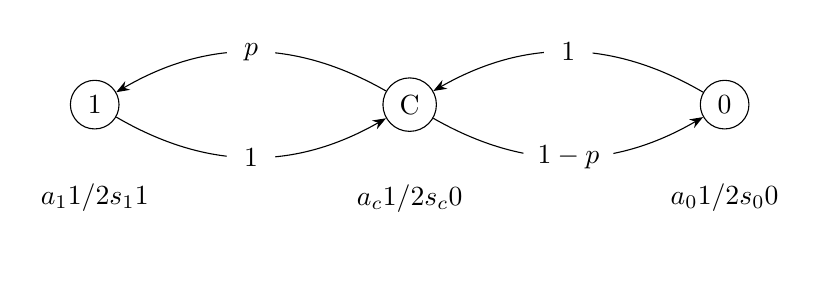
\begin{tikzpicture}
      \begin{scope}[every node/.style={circle,draw}]
        \node (C) at (0,0) [label=below:$a_c \equal 1/2\comma s_c \equal 0$]{C};
        \node (1) at (-4,0)[label=below:$a_1 \equal 1/2\comma s_1 \equal 1$]{1};
        \node (2) at (4,0) [label=below:$a_0 \equal 1/2\comma s_0 \equal 0$]{0};
      \end{scope}
      \begin{scope}[>={Stealth[black]},
        every node/.style={fill=white,circle},
        every edge/.style={draw=black}]
        \path [->] (C) edge[bend right] node {$p$} (1);
        \path [->] (C) edge[bend right] node {$1-p$} (2);
        \path [->] (1) edge[bend right] node {$1$} (C);
        \path [->] (2) edge[bend right] node {$1$} (C);
      \end{scope}
    \end{tikzpicture}
    \vspace{-10mm}
    \caption{The Lower Bound Instance} \label{fig:lb_instance}
  \end{figure}
  %
\end{proof}
%
It follows by Lemma~\ref{l:reduction} that in order to prove Theorem~\ref{t:lower_bound} we
just need to prove the following claim.
\begin{claim}\label{cl:fixed_p}
  For any estimator $\theta = (\theta_t)_{t=1}^\infty$
  there exists a fixed $p \in [0,1]$ such that
  \(
    \lim_{t \to \infty} t^{1+c} \Expnew{p}{|\theta_t - p} > 0.
  \)
\end{claim}
The above claim states that for any estimator $\theta=(\theta_t)_{t=1}^\infty$,
we can inspect the functions $\theta_t: \{0,1\}^t \mapsto [0,1]$ and then choose
a $p \in [0,1]$ such that the function $E_p[|\theta_t-p|]= \Omega(1/t^{1+c})$. As
a result, we have reduced the construction of a lower bound concerning the round
complexity of a dynamical process to a lower bound concerning the sample complexity of
estimating the parameter $p$ of a Bernoulli distribution. The claim follows by
Lemma~\ref{l:estimation_lower_bound} which we present at the end of the section.

At this point we should mention that it is known
that $\Omega(1/\eps^2)$ samples are needed to estimate the parameter $p$
of a Bernoulli random variable within additive error $\eps$.
Another well-known result is that taking the average of the samples
is the \emph{best} way to estimate the mean of a Bernoulli random variable.
These results would indicate that the best possible rate of convergence
for an \emph{opinion dependent dynamics} would be $O(1/\sqrt{t})$.
However, there is some fine print in these results which does not allow us
to use them. In order to explain the various limitations of
these methods and results we will briefly discuss some of them.

Perhaps the oldest sample complexity lower bound for estimation problems
is the well-known Cramer-Rao inequality.
Let the function $\theta_t: \{0,1\}^t \mapsto [0,1]$ such that $E_p[\theta_t]=p$ for
all $p \in [0,1]$, then
\begin{equation}\label{eq:crlb}
  \Expnew{p}{(\theta_t - p)^2} \geq \frac{p(1-p)}{t}.
\end{equation}
Since $\Expnew{p}{|\theta_t - p|}$ can be lower bounded
by $\Expnew{p}{(\theta_t - p)^2}$ we can apply the Cramer-Rao inequality and
prove our claim in the case of \emph{unbiased} estimators, $E_p[\theta_t]=p$
for all $t$. Obviously, we need to prove it for any estimator $\theta$, however
this is a first indication that our claim holds.
%Simply setting $p=1/2$ in inequality (\ref{eq:crlb}) would give us a
%$p$ satisfying the requirements of Claim~\ref{cl:fixed_p}.
%The problem with this lower bound is that the assumption that the estimator
%is unbiased is considered rather restrictive and unrealistic even in
%the statistics literature in the sense that many efficient practical
%estimators are not unbiased.  Thus, we would like to get a lower bound
%with minimal assumptions about the estimator.

To the best of our knowledge, sample complexity lower bounds without
assumptions about the estimator are given as lower bounds for the
\emph{minimax risk}, which was defined
\footnote{
  Although the minimax risk is defined for any estimation problem and loss
  function, for simplicity, we write the minimax risk for estimating the mean
  of a Bernoulli random variable.}
by Wald in \cite{Wal39} as
\[
  \min_{\theta_t} \max_{p\in[0,1]} \Expnew{p}{|\theta_t - p|}.
\]
\noindent Minimax risk captures the idea that after we pick the best possible
algorithm, an adversary inspects it and picks the worst possible
$p \in[0,1]$ to generate the samples that our algorithm will get as input.
The methods of Le'Cam, Fano, and Assouad are well-known
information-theoretic methods to establish lower bounds for the minimax risk.
For more on these methods see \cite{Yu97,Tsy08} and the
very good lecture notes of Duchi, \cite{duchi_stats311}.
As we stated before, it is well known that the minimax risk for the
case of estimating the mean of a Bernoulli is lower bounded by
$\Omega(1/\sqrt{t})$ and this lower bound can be established
by Le Cam's method.
In order to show why such arguments do no work for our purposes
we shall sketch how one would apply Le Cam's method to get this lower bound.
To apply Le Cam's method, one typically chooses two Bernoulli distributions
whose means are far but their total variation distance is small.
Le Cam showed that when two distributions are close in total variation then
given a sequence of samples $X_1, \ldots, X_t$ it is hard to tell whether
these samples were produced by $P_1$ or $P_2$. The hardness of this \emph{testing}
problem implies the hardness of \emph{estimating} the parameters of
a family of distribution.
For our problem the two distributions would be $B(1/2 - 1/\sqrt{t})$
and $B(1/2 + 1/\sqrt{t})$. It is not hard to see that their total variation
distance is at most $O(1/t)$, which implies a lower bound
$\Omega(1/\sqrt{t})$ for the minimax risk. The problem here is that
the parameters of the two distributions depend on the number of
samples $t$. The more samples the algorithm gets to see, the closer
the adversary takes the $2$ distributions to be.
For our problem we would like to \emph{fix} an instance and then argue
about the rate of convergence of any algorithm on this instance.
Namely, having an instance that depends on $t$ does not work for us.

Trying to get a lower bound without assumptions about the estimators
while respecting our need for a fixed (independent of $t$) $p$ we prove
Lemma~\ref{l:estimation_lower_bound}.
In fact, we show something stronger:
for \emph{almost all} $p \in [0,1]$, any estimator $\theta$ cannot
achieve rate $o(1/t^{1+c})$.
More precisely,  suppose we select a $p$ uniformly at
random in $[0,1]$ and run the estimator $\theta$ with samples from the
distribution $B(p)$, then with probability $1$ the error rate $\Expnew{p}{|\theta_t  - p |} \in
\Omega(1/t^{1+c})$. Although we do not show the sharp lower bound
$\Omega(1/\sqrt{t})$ we prove that no exponential convergence rate
is possible and we remark that our proof is fairly simple, intuitive,
and could be of independent interest.
%
% Finally, while we do not preclude the possibility of similar results to exist
% in the statistics literature,

\begin{lemma}\label{l:estimation_lower_bound}
  Let a Bernoulli estimator $\theta=(\theta_t)_{t=1}^\infty$
  with error rate $\Expnew{p}{|\theta_t  - p |}$.
  For any $c>0$, if we select $p$ uniformly at random in $[0,1]$ then
   \(\lim_{t\to \infty} t^{1+c} \Expnew{p}{|\theta_t  - p |} > 0\) with
   probability $1$.
\end{lemma}
\begin{proof}
  Let an estimator $\theta = \{\theta_t\}_{t=1}^{\infty}$, where
  $\theta_t: \{0,1\}^t\mapsto [0,1]$.  The function $\theta_t$ can have at most
  $2^t$ different values. Without loss of generality we assume that
  $\theta_t$ takes the same value $\theta_t(x)$ for all $x \in \{0,1\}^t$
  with the same number of $1$'s. For example,
  $\theta_3(\{1,0,0\})=\theta_3(\{0,1,0\})=\theta_3(\{0,0,1\})$.
  This is due to the fact that for any $p \in[0,1]$,
  %
  \[
    \sum_{0 \leq i \leq t} \sum_{\norm{1}{x} = i} \lp| \theta_t(x) - p \rp|
    p^i (1-p)^{t-i} \geq \sum_{0 \leq i \leq t} \binom{t}{i} \lp|
    \frac{\sum_{\norm{1}{x} = i} \theta_t(x)}{\binom{t}{i}}  - p \rp| p^i
    (1-p)^{t-i}.
  \]
  %
  For any estimator $\theta$ with error rate $\Expnew{p}{|\theta_t  - p |}$ there exists another
  estimator $\theta'$ that satisfies the above property and
  $\Expnew{p}{|\theta_t'  - p |} \leq \Expnew{p}{|\theta_t  - p |}$ for all $p \in [0,1]$.
  Thus we can assume that $\theta_t$ takes at most $t+1$ different
  values.
  %
  Let $A$ denote the set of $p$ for which the estimator has error
  rate $o(1/t^{1+c})$, that is
  %
  \[
    A= \{p\in [0,1]: \lim_{t \to \infty} t^{1+c}\Expnew{p}{|\theta_t  - p |}=0\}
  \]
  We show that if we select $p$ uniformly at random in $[0,1]$ then
  $\Prob{p \in A} = 0$.  We also define the set
  \[
    A_k=\{p\in [0,1]: \text{for all }t \geq k,~ t^{1+c}\Expnew{p}{|\theta_t  - p |}\leq 1\}
  \]
  %
  Observe that if $p \in A$ then there exists $t_p$ such that
  $p \in A_{t_p}$, meaning that
  $A \subseteq \cup_{k=1}^{\infty}A_k$.  As a result,
  \[
    \Prob{p \in A} \leq \Prob {p \in\bigcup_{k=1}^{\infty}A_k} \leq
    \sum_{k=1}^{\infty}\Prob{p \in A_k}
  \]
  %
  To complete the proof we show that $\Prob{p \in A_k}=0$ for all $k$.
  Notice that $p \in A_k$ implies that for $t \geq k$, the estimator
  $\theta$ must always have a value $\theta_t(i)$ close to $p$.
  Using this intuition we define the set
  \[
    B_k = \{p \in [0,1]: \text{for all
    }t\geq k,~ t^{1+c}\min_{0\leq i \leq t}|\theta_t(i)-p| \leq 1\}
  \]
  %
  We now show that $A_k \subseteq B_k$.
  Since $p \in A_k$ we have that for all $t\geq k$
  \[
    t^{1 + c} \min_{0 \leq i \leq t} \lp| \theta_t(i) - p \rp|
    \sum_{i=0}^t \binom{t}{i} p^i (1-p)^{t-i}
    \leq
    t^{1 + c} \sum_{i=0}^t \binom{t}{i} \lp| \theta_t(i) - p \rp| p^i (1-p)^{t-i}
    = t^{1+c} \Expnew{p}{|\theta_t  - p |}
    \leq
    1/2.
  \]
  %
  Thus, $\Prob{p \in A_k} \leq \Prob{p \in B_k}$.
  We write the set $B_k$ as \(
    B_k = \bigcap_{t=k}^{\infty}\{p \in [0,1]:~ \min_{0 \leq
      i \leq t} |\theta_t(i)-p|\leq 1/t^{1+c}
    \}.
  \)
  %
  As a result,
  \(
    \Prob{p \in B_k}
    \leq \Prob{\min_{0 \leq i \leq t}|\theta_t(i)-p| \leq 1/t^{1+c} },
    \text{for all } t \geq k.
  \)
  \begin{figure}
    \centering
    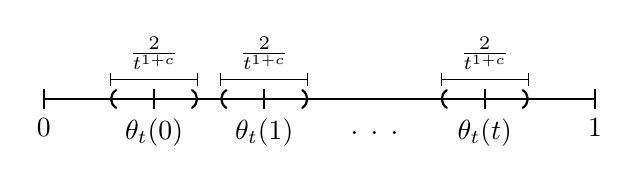
\begin{tikzpicture}[scale=7]
      \draw[-, thick] (0,0) -- (1,0);
      \foreach \x/\xtext in {0/0,0.2/$\theta_t(0)$,0.4/$\theta_t(1)$,0.8/$\theta_t(t)$,1}
      \draw[thick] (\x,0.5pt) -- (\x,-0.5pt) node[below] {\xtext};
      %\draw (0.2,0.5pt) node[above] {$c$};
      \draw[(-), thick, black] (0.12,0) -- (0.28,0);
      \draw[(-), thick, black] (0.32,0) -- (0.48,0);
      \draw (0.6,-1.2pt) node[below] {. . . };
      \draw[(-), thick, black] (0.72,0) -- (0.88,0);
      \draw[|-|] (0.12,1pt) -- (0.28,1pt) node[midway, above] {$\frac{2}{t^{1+c}}$};
      \draw[|-|] (0.32,1pt) -- (0.48,1pt) node[midway, above] {$\frac{2}{t^{1+c}}$};
      \draw[|-|] (0.72,1pt) -- (0.88,1pt) node[midway, above] {$\frac{2}{t^{1+c}}$};
      %\draw (-0.25,0) node {At time $t$};
    \end{tikzpicture}
    \caption{Estimator output at time $t$} \label{fig:estimator}
  \end{figure}
  Each value $\theta_t(i)$ \enquote{covers} length $1/t^{1+c}$ from
  its left and right, as shown in Figure~\ref{fig:estimator},
  and since there are at most $t+1$ such values
  we have for all $t \geq k$ the set
  \(
    \{
    p \in [0,1]:\ {\min_{0 \leq i \leq t} |\theta_t(i)-p| \leq 1/t^{1+c} }
    \}
    =
    \bigcup_{i=0}^t
    \lp(
    \theta_t(i) - \frac{1}{t^{1+c}},\ \theta_t(i) + \frac{1}{t^{1+c}}
    \rp).
  \)
  For each interval in the above union we have that
  $\Prob{|\theta_t(i)-p| \leq 1/t^{1+c}}\leq 2/t^{1+c}$
  and by the union bound we get
  $\Prob{p \in B_k} \leq 2(t+1)/t^{1+c}$, for all $t \geq k$.
  We conclude that $\Prob{p \in B_k} =0$.
\end{proof}

%\begin{remark}\label{r:lower_bound_no-regret}
%  The only point that we use that
%  the update rules are \emph{opinion dependent} is in Lemma~\ref{l:reduction}.
%  It is not difficult to see that the reduction still holds if the update rules
%  also depend on the indices of the neighbors that an agent meets.
%  As a result, Theorem~\ref{t:lower_bound} still applies.
%\end{remark}

\section{An Update Rule with Fast Convergence Rate}\label{s:cc_convergence}

We already discussed that the reason that opinion dependent dynamics suffer slow
convergence is that the update rule depends only on the expressed opinions.
Based on works for asynchronous distributed minimization algorithms \cite{BT97,CC16},
we provide an update rule showing that information about the
graph $G$ combined with agents that do not act selfishly can restore the
fast convergence rate.
Our update rule, depends not only on the expressed opinions of the
neighbors that an agent $i$ meets but also on the $i$-th row of matrix $P$.
In update rule (\ref{alg:cc_upper}), each agent stores the
\emph{most recent} opinions of the random neighbors that she meets in an array
and then updates her opinion according to their weighted sum
(each agent knows row $i$ of $P$). For a given instance
$I=(P,s,\alpha)$ we call the produced dynamics \emph{Row Dependent dynamics}
and it is defined in Dynamics~\ref{alg:influence_dependent}.

The problem with this approach is that the opinions of the neighbors
that she keeps in her array are \emph{outdated}, i.e. the opinion of
a neighbor of agent $i$ has changed since their last meeting.
The good news are that as long as this outdatedness
is bounded we can still achieve fast convergence to the
equilibrium.  By bounded outdatedness we mean that there exists a
number of rounds $B$ such that all agents have met all their neighbors
at least once from $t-B$ to $t$. The latter is formally stated in
Lemma~\ref{l:outdatedness_induction} and its proof can be found
Appendix~\ref{app:s:cc_convergence}.

\begin{remark}
  %It is necessary that each agent $i$ \enquote{knows} the row $i$ of matrix $P$ for
  %this update rule to work.
  Update rule~(\ref{alg:cc_upper}), apart from the opinions
  and the indices of the neighbors that an agent meets,
  also depends on the the exact values of the weights $p_{ij}$ and that is
  why \emph{Row Dependent dynamics} converge fast. We mention that the lower bound of
  Section~\ref{s:lower_bound} still holds even if the agents also use the indices
  of the neighbors that they meet to update their opinion, since
  Lemma~\ref{l:reduction} can be easily modified to
  cover this case. The latter implies that any update rule that
  ensures fast convergence must require that each agent
  $i$ is \emph{aware} of the $i$-th row of matrix $P$.

\end{remark}
\vspace{-5mm}
\begin{algorithm*}
  \caption{Row Dependent dynamics}
  \label{alg:influence_dependent}
  \begin{algorithmic}[1]
    \STATE Initially $x_i(0) = s_i$ for all agent $i$.
    \STATE Each agent $i$ keeps an array $M_i$ of length $|N_i|$,
    randomly initialized.
    \STATE At round $t\geq 0$ each agent $i$:
    \bindent
    \STATE Meets neighbor with index $W_i^t$, $\Prob{W_i^t=j}=p_{ij}$.
    \STATE Suffers cost \((1-\alpha_i) (x_i(t) - x_{W_i^t}(t))^2 + a_i (x_i(t) - s_i)^2\)
    and learns $(x_{W_i^t}(t),W_i^t)$.
    \STATE Updates her array $M_i$ and opinion:
    $
    M_i[W_i^t] \gets x_{W_i^t}(t),\quad
    x_i(t+1) = (1-\alpha_i)\sum_{j \in N_i} p_{ij} M_i[j] + \alpha_i s_i
    $
    \inlineequation[alg:cc_upper]{}
    \eindent
  \end{algorithmic}
\end{algorithm*}

%In \cite{BT97}, they show a convergence rate guarantee for
%\ref{alg:cc_upper} assuming that there exists a such a window $B$.
%In the  following we briefly summarize their result.  For completeness we
%give here a prove tailored for our purposes.
%Using a simple induction we get that bounded outdatedness
%preserves the fast convergence.  Its simple proof can be found in
\begin{replemma}{l:outdatedness_induction}
  Let $\rho = \min_i a_i$, and $\pi_{ij}(t)$ be the most recent round
  before round $t$, that agent $i$ met her neighbor $j$.
  If for all $t\geq B$, $t-B \leq \pi_{ij}(t)$ then, for
  all $t \geq k B$,
  \(\norm{\infty}{x(t) - x^*} \leq (1-\rho)^k\).
\end{replemma}

In our randomized setting there does not exist a fixed length window $B$
that satisfies the requirements of Lemma~\ref{l:outdatedness_induction}.
However we can select a length value such that the requirements hold with high probability.
To do this observe that agent $i$ simply needs to wait to meet the neighbor
$j$ with the smallest weight $p_{ij}$. Therefore, after
$\log(1/\delta)/\min_{j} p_{ij}$ rounds we have that with probability at least
$1-\delta$ agent $i$ met all her neighbors at least once.
Since we want this to be true for all agents
we shall roughly take $B = 1/\min_{p_{ij} > 0} {p_{ij}}$.
In Section~\ref{app:s:cc_convergence} of the Appendix we give the detailed
argument that leads to the Theorem~\ref{t:exponential_update_rule},
showing that the convergence rate of update rule (\ref{alg:cc_upper}) is fast.

\begin{reptheorem}{t:exponential_update_rule}
  Let $I = (P,s, \alpha)$ be an instance of the opinion formation
  game of Definition~\ref{d:random_game} with equilibrium
  $x^* \in [0,1]^n$ and let $\rho = \min_{i \in V} a_i$.
  The opinion vector $x(t)\in[0,1]^n$ produced by
  update rule~(\ref{alg:cc_upper}) after $t$ rounds satisfies
  \(
    \Exp{\norm{\infty}{x(t) - x^*}}
    \leq
    2\exp(- \rho  \min_{ij} p_{ij} \sqrt{t}/(4\ln(nt)) ).
  \)
\end{reptheorem}


\bibliographystyle{alpha}
\bibliography{refs}

\clearpage
\appendix

\section{The Convergence Rate of FTL Dynamics}\label{app:s:fictitious_convergence}
We give here the proof of the following technical lemma that we used to derive
an upper bound on the rate of convergence of the fictitious play dynamics in
Section~\ref{s:fictitious_convergence}.  We restate Lemma~\ref{l:recursion_upper_bound} for
completeness.
\repeatlemma{l:recursion_upper_bound}
% \begin{lemma}
%   Let $e(t)$ be a function satisfying the recursion
%   \[
%     e(t) =
%     \delta(t) + (1-\rho)\frac{\sum_{\tau=0}^{t-1}e(\tau)}{t}
%     \text{ and } e(0)=\|x^0 - x^*\|_{\infty},
%   \]
%   where \(\delta(t) = \sqrt{\frac{\ln(D t^2)}{t}} \), \(\delta(0) = 0 \),
%   and $D > \me^2$ is a positive constant.  Then
%   \(
%     e(t) \leq
%     \sqrt{2 \ln(D)} \frac{(\ln t)^{3/2}}{t^{\min(\rho,\, 1/2)}}.
%   \)
% \end{lemma}
\begin{proof}
  Observe that for all $t\geq 0$ the function $e(t)$ the following recursive
  relation
  \begin{equation}\label{eq:recursion}
    e(t+1) = e(t) \lp(1 - \frac{\rho}{t+1} \rp)
    + \delta(t+1)-\delta(t) + \frac{\delta(t)}{t+1}\\
  \end{equation}
  For $t=0$ we have that
  \begin{equation}\label{eq:recursion_zero}
    e(1) = (1- \rho)e(0) + \delta(1) = (1 -\rho)e(0) + \sqrt{\ln D}
  \end{equation}
  Observe that for $D>\me^2$, $\delta(t)$ is decreasing for all $t\geq 1$.
  Therefore, \(
    \delta(t+1)-\delta(t) + \frac{\delta(t)}{t+1}\leq \frac{\delta(t)}{t+1} \)
  and from equations (\ref{eq:recursion}) and (\ref{eq:recursion_zero})
  we get that for all $t\geq 0$
  \[
    e(t+1) \leq
    e(t) \lp(1 - \frac{\rho}{t+1} \rp) +
    \frac{\sqrt{\ln(D (t+1)^2)}}{(t+1)^{3/2}}
    \leq
    e(t) \lp(1 - \frac{\rho}{t+1} \rp) +
    \frac{\sqrt{2 \ln(D (t+1))}}{(t+1)^{3/2}}
  \]
  Now let \(g(t) = \frac{\sqrt{2 \ln(D t)}}{t^{3/2}} \) to obtain
  for all $t\geq 1$
  \begin{align*}
    e(t)
    &\leq
    (1-\frac{\rho}{t})e(t-1) + g(t)\\
    &\leq
    (1-\frac{\rho}{t})(1-\frac{\rho}{t-1})e(t-2)
    + (1-\frac{\rho}{t})g(t-1) + g(t)\\
    &\leq
    (1-\frac{\rho}{t})\cdots (1-\rho)e(0)
    + \sum_{\tau=1}^t g(\tau)\prod_{i=\tau+1}^t(1-\frac{\rho}{i})\\
    &\leq
    \frac{e(0)}{t^\rho}
    + \sum_{\tau=1}^tg(\tau)e^{-\rho\sum_{i=\tau+1}^t\frac{1}{i}}\\
    &\leq
    \frac{e(0)}{t^\rho}
    + \sum_{\tau=1}^tg(\tau)e^{-\rho(H_t-H_{\tau})}\\
    &\leq
    \frac{e(0)}{t^\rho}
    + e^{-\rho H_t}\sum_{\tau=1}^tg(\tau)e^{\rho H_{\tau}}\\
    &\leq
    \frac{e(0)}{t^\rho}
    + \frac{\sqrt{2}}{t^\rho}
    \sum_{\tau=1}^t\tau^\rho\frac{\sqrt{\ln (D \tau)}}{\tau^{3/2}}\\
    &\leq
    \frac{e(0)}{t^\rho}
    + \frac{\sqrt{2 \ln D }}{t^\rho}
    \sum_{\tau=1}^t\frac{\sqrt{\ln \tau}}{\tau^{3/2-\rho}}
  \end{align*}
  We observe that
  \begin{equation}\label{eq:integral_upper_bound}
    \sum_{\tau=1}^t
    \frac{\sqrt{\ln \tau}}{\tau^{3/2-\rho}}
    \leq
    \int_{\tau=1}^t \frac{\sqrt{\ln\tau}}{\tau^{3/2-\rho}}\d \tau
  \end{equation}
  since, \(\tau \mapsto \frac{\sqrt{\ln\tau}}{\tau^{3/2-\rho}}\)
  is a decreasing function of $\tau$ for all $\rho \in[0,1]$.

  \begin{itemize}
    \item If
      $\rho\leq 1/2$ then
      \[
        \int_{\tau=1}^t \tau^\rho\frac{\sqrt{\ln \tau}}{\tau^{3/2}}\d\tau
        \leq
        \sqrt{\ln t }
        \int_{\tau=1}^t
        \frac{1}{\tau}\d\tau = (\ln t)^{3/2}
      \]
    \item If $\rho > 1/2$ then\\
      \begin{align*}
        \int_{\tau=1}^t
        \tau^\rho\frac{\sqrt{\ln \tau}}{\tau^{3/2}}\d\tau
        &=
        \int_{\tau=1}^t \tau^{\rho-1/2}\frac{\sqrt{\ln \tau}}{\tau}d\tau \\
        &=
        \frac{2}{3} \int_{\tau=1}^t
        \tau^{\rho-1/2}((\ln \tau)^{3/2})'\d\tau \\
        &=
        \frac{2}{3}t^{\rho - 1/2}(\ln t)^{3/2} - (\rho-1/2)\frac{2}{3}
        \int_{\tau=1}^t \tau^{\rho-3/2}(\ln \tau)^{3/2}\d\tau \\
        &\leq \frac{2}{3} t^{\rho - 1/2}(\ln t)^{3/2}
      \end{align*}
  \end{itemize}
\end{proof}

\begin{theorem}\label{thm:convergence}
  Let $I = (P,s, \alpha)$ be any instance of the opinion formation
  game of Definition~\ref{d:random_game} with equilibrium
  $x^* \in [0,1]^n$.  The opinion vector $x(t)$ produced by
  update rule~\ref{eq:fictitious_play}
  after $t$ rounds satisfies
  \[
    \Expnew{}{\norm{\infty}{x(t) - x^*}} \leq
    C \sqrt{\log n}\frac{(\log t)^{3/2}}{t^{\min(1/2,\rho)}},
  \]
  where $\rho = \min_{i \in V} a_i$ and $C$ is a universal constant.
\end{theorem}

\begin{proof}
By Lemma~\ref{l:recursive_equation} we have that for all $t\geq 1$ and $p \in [0,1]$,
\[\Prob{\norm{\infty}{x(t)-x^*} \leq e_p(t)} \geq 1-p\]
where $e_p(t)$ is the solution of the recursion, $e_p(t) =\delta(t) + (1-\rho)\frac{\sum_{\tau=0}^{t-1}e_p(\tau)}{t}$ with
$\delta(t)=\sqrt{ \frac{\log(\pi^2 n t^2/(6 p))}{t}}$. Setting $p=\frac{1}{12\sqrt{t}}$ we have that
\[\Prob{\norm{\infty}{x(t)-x^*} \leq e(t)} \geq 1-\frac{1}{12\sqrt{t}}\]
where $e(t)$ is the solution of the recursion $e(t) =\delta(t) + (1-\rho)\frac{\sum_{\tau=0}^{t-1}e_p(\tau)}{t}$ with
$\delta(t)=\sqrt{\frac{\log(2\pi^2 n t^{2.5})}{t}}$. Since $2\pi^2 \geq e^{2.5}$, Lemma~\ref{l:recursion_upper_bound} applies and
$e(t)\leq C\sqrt{\log n}\frac{\log t^{3/2}}{t^{\min(\rho,1/2)}}$ for some universal constant $C$. Finally,
\[\Expnew{}{\norm{\infty}{x(t) - x^*}} \leq \frac{1}{12\sqrt{t}} + (1-\frac{1}{12\sqrt{t}})C\sqrt{\log n}\frac{(\log t)^{3/2}}{t^{\min(\rho,1/2)}}
\leq (C+\frac{1}{12})\sqrt{\log n}\frac{(\log t)^{3/2}}{t^{\min(\rho,1/2)}}\]
\end{proof}

\section{FTL dynamics has no-regret}\label{app:s:fictitious_noregret}
We prove here Lemma~\ref{l:y_t}, which we restate for
convenience.
\begin{lemma}
Let $\{b_t\}_{t=0}^\infty$ be an arbitrary sequence with $b_t \in [0,1]$. Let $y_t = \argmin_{x \in [0,1]}\sum_{\tau=0}^tf(x_,b_\tau)$
then for all $t$,
\[
\sum_{\tau=0}^t f(y_\tau,b_\tau) \leq \min_{x \in [0,1]}\sum_{\tau = 0}^tf(x,b_\tau)
\]
\end{lemma}
\begin{proof}By definition of $y_t$,
  $\sum_{\tau=0}^t f(y_t,b_\tau)=\min_{ x \in [0,1]} \sum_{\tau=0}^t f(x,b_\tau)$, so
  \begin{align*}
    \sum_{\tau=0}^t f(y_\tau,b_\tau) - \min_{ x \in [0,1]} \sum_{\tau=0}^t f(x,b_\tau) &=
    \sum_{\tau=0}^t f(y_\tau,b_\tau) - \sum_{\tau=0}^t f(y_t,b_\tau)\\
    &= \sum_{\tau=0}^{t-1} f(y_\tau,b_\tau) - \sum_{\tau=0}^{t-1} f(y_t,b_\tau)\\
    &\leq \sum_{\tau=0}^{t-1} f(y_\tau,b_\tau) - \sum_{\tau=0}^{t-1} f(y_{t-1},b_\tau)\\
%    &= \sum_{\tau=0}^{t-2} f(y_\tau,b_\tau) - \sum_{\tau=0}^{t-2}f(y_{t-1},b_\tau)
  \end{align*}
  The last inequality follows by the fact that $y_{t-1} = \argmin_{x \in [0,1]}\sum_{\tau=0}^{t-1}f(x_,b_\tau)$
  Inductively, we prove that $\sum_{\tau=0}^t f(y_\tau,b_\tau) \leq \min_{ x \in [0,1]} \sum_{\tau=0}^t f(x,b_\tau)$.
\end{proof}

We next prove Lemma~\ref{l:no_regret_lemma} which we combine with
Lemma~\ref{l:y_t} to show that the update rule~\ref{eq:fictitious_play}
ensures no regret for the agents. We first restate the Lemma for
convenience.
\begin{lemma}
  For all $t\geq 0$,
  \(
    f(x_t,b_t) \leq f(y_t,b_t) + 2\frac{1-\alpha}{t+1} +
    \frac{(1-\alpha)^2}{(t+1)^2}
  \).
\end{lemma}
\begin{proof}
  We first prove that for all $t$,
  \begin{equation}\label{eq:abs_value}
    \lp|x_t - y_t \rp| \leq \frac{1-\alpha}{t+1}.
  \end{equation}
  By definition
  \(x_t = \alpha s + (1-\alpha)\frac{\sum_{\tau = 0}^{t-1} b_\tau}{t}\)
  and
  \( y_t = \alpha s + (1-\alpha)\frac{\sum_{\tau = 0}^t b_\tau}{t+1}\).
  \begin{align*}
    \lp|x_t - y_t\rp|
    &=
    (1-\alpha)\lp|\frac{\sum_{\tau = 0}^{t-1}b_\tau}{t}
    - \frac{\sum_{\tau = 0}^t b_\tau}{t+1}\rp|\\
    &=
    (1-\alpha)\lp|\frac{\sum_{\tau = 0}^{t-1}b_\tau -tb_t}{t(t+1)}\rp|\\
    &\leq
    \frac{1-\alpha}{t+1}
  \end{align*}
  The last inequality follows from the fact that $b_\tau \in [0,1]$.
  We now use inequality~(\ref{eq:abs_value}) to bound the difference
  \( f(x_t,b_t) - f(y_t,b_t) \).
  \begin{align*}
    f(x_t,b_t)
    &=
    \alpha(x_t - s)^2 + (1 - \alpha)(x_t - y_t)^2 \\
    &\leq
    \alpha(y_t - s)^2 + 2\alpha\lp|y_t -
    s\rp|\lp|x_t - y_t\rp| + \alpha \lp|x_t - y_t\rp|^2 \\
    &\quad + (1-\alpha)(y_t - y_t)^2 +
    2(1-\alpha)\lp|y_t - y_t\rp|\lp|x_t-y_t\rp| + (1 - \alpha)\lp|x_t - y_t\rp|^2\\
    &\leq
    f(y_t,b_t) + 2\lp|x_t - y_t\rp| + \lp|y_t - x_t\rp|^2\\
    &\leq
    f(y_t,b_t) + 2\frac{1-\alpha}{t+1} + \frac{(1-\alpha)^2}{(t+1)^2}
  \end{align*}
\end{proof}

\section{Faster Update Rule}\label{app:s:cc_convergence}
We are now going to state and prove a series of Lemmas that culminate in
the proof of Lemma~\ref{l:cc_convergence}. We first turn our attention to
the problem of calculating the size of window $B$, such that with high probability
all agents have outdateness at most $B$.
We first state a useful fact concerning the coupons collector problem.

\begin{lemma}\label{l:coupons_lemma}
Suppose that the collector picks coupons with mixed
probabilities, where $n$ is the number of distinct coupons.
Let $w$ be the minimum of these probabilities.
If he selects $\ln n/w+ c/w$ coupons, then:
$$
\Prob{\text{collector hasn't seen all coupons}} \leq \frac{1}{\me^c}
$$
\end{lemma}

For convenience of reasoning, we will divide the time in "epochs".
The length of each epoch is $B$, so times $1$ to $B$ belong to the first
epoch etc.
The next lemma is a calculation of the appropriate size of $B$.
\begin{lemma}
Suppose we run Algorithm~\ref{alg:cc_upper} for $t$ rounds. If the size of
each epoch is
\[
B = \frac{2}{\min_{ij}p_{ij}}\ln \frac{nt}{p}
\]
then with probability at least $1-p$ all agents pick all their neighbours
at least once in every epoch.
\end{lemma}
\begin{proof}
In our setting, coupon $i$ corresponds to the selection of neighbour $i$. Each node is a
collector and wants to gather all $n-1$ coupons during each epoch.
Suppose $d = \max_i d_i$ is the maximum degree of the graph.
Then, if we set  $c = \ln (\frac{nt}{p})$ , using Lemma~\ref{l:coupons_lemma}
we get that a node hasn't seen at least one neighbour after $c/w + \ln d/w$ samples
with probability at most $\frac{p}{nt}$. This means that if we set
$D = c/w + \ln d/w =  \ln \frac{nt}{p}/w +  \ln d/w \geq 2/w\ln\frac{nt}{p} $ when $p$ is
small enough, then the probability that a specific agent at a specific epoch hasn't collected
all neighbouring opinions at least once is at most $\frac{p}{nt}$. By a simple union bound argument,
we get that all agents have seen all their neighbours during all epochs
 with probability at least $1 - p$.
\end{proof}
Since all neighbours are picked at least once during each epoch,
the outdatedness of each agent is at most twice the length of the
epoch. We now show Lemma~\ref{l:outdatedness_induction}
from which we get that bounded outdatedness preserves the exponential
convergence.
\begin{lemma}
  Let $\rho = \min_i a_i$, and $\pi_{ij}(t) \in \N$ be the most recent round
  before round $t$, that agent $i$ met agent $j$.
  If for all $t\geq B$, $t-B \leq \pi_{ij}(t) \leq t-1$ then, for
  all $t \geq k B$,
  \(\norm{\infty}{x(t) - x^*} \leq (1-\rho)^k\).
\end{lemma}
\begin{proof}
  To prove our claim we use induction on $k$. For the induction base $k=1$,
  \begin{align*}
    |x_i(t) - x_i^*|
    =
    |(1-\alpha_i)\sum_{j \in N_i}p_{ij}(x_j(\pi_{ij}(t)) -x_j^*)|
    \leq
    (1-\alpha_i)\sum_{j \in N_i}p_{ij}|(x_j(\pi_{ij}(t))-x_j^*)|\leq (1-\rho)
  \end{align*}
  From the induction hypothesis we have for $\pi_{ij}(t) \geq (k-1)B$,
  that $|x_j(\pi_{ij}(t))-x_j^*| \leq (1-\rho)^{k-1}$.
  For $k\geq 2$, we again have that
  $|x_i(t) - x_i^*|\leq (1-\rho)\sum_{j \in N_i}p_{ij}|(x_j(\pi_{ij}(t))-x_j^*)|$.
  Since $t-B \leq \pi_{ij}(t)$ and $t\geq kB$, we have
  that $\pi_{ij}(t) \geq (k-1)B$ and the induction hypothesis applies.
\end{proof}

Combining this with Lemma~\ref{l:outdatedness_induction} we have
the following.
\begin{corollary}\label{cor:window}
If we run Algorithm~\ref{alg:cc_upper} for $t$ rounds, then with probability at least
$1-p$
$$ \norm{\infty}{x^{t}-x^*} \leq (1-\rho)^{\frac{t}{2B}}
\leq \exp \lp(-\frac{\rho t\min_{ij}p_{ij}}{2\ln( \frac{nt}{p})} \rp)$$
\end{corollary}
We now prove Lemma~\ref{l:cc_convergence} using the previous results.
\repeatlemma{l:cc_convergence}
\begin{proof}
Let $u(t) = \norm{\infty}{x^t-x^*}$ and $w = \min_{ij}p_{ij}$.
From Corollary~\ref{cor:window} we obtain:
$$ \Prob{u(t) >\exp\lp(-\frac{\rho wt}{2\ln( \frac{nt}{p})} \rp)} \leq p $$
for every probability $p \in [0,1]$. Also, since all the
parameters of the problem lie in $[0,1]$, we have
$$\Exp{u(t)|u(t) > r} \leq 1$$
Now, by the conditional expectations identity, we get:
\begin{align*}
\Exp{u(t)} &= \Exp{u(t)|u(t) > r}\Prob{u(t) > r} +\Exp{u(t)|u(t) \leq r}\Prob{u(t) \leq r}\\
&\leq p + r
\end{align*}
where $r = \exp \lp(-\frac{\rho wt}{2\ln( \frac{nt}{p})}\rp)$.
If we set $p = \exp \lp(-\frac{\rho w\sqrt{t}}{2\ln nt}\rp)$, then:
$$
\Exp{u(t)} \leq \exp \lp(-\frac{\rho w\sqrt{t}}{2\ln nt}\rp)
+ \exp \lp(-\frac{\rho wt}{2\ln( \frac{nt}{p})}\rp)
$$
We now evaluate $r$ for our choice of probability $p$:
\begin{align*}
r
&= \exp \lp(-\frac{\rho wt}{2\ln\lp( \frac{nt}{p}\rp)} \rp)\\
&= \exp \lp(-\frac{\rho wt}{2\ln\lp( \frac{nt}{\exp \lp(-\frac{\rho w\sqrt{t}}{2\ln nt}\rp) }\rp) } \rp) \\
&= \exp \lp(-\frac{\rho wt}{2\ln nt + 2\frac{\rho w\sqrt{t}}{2\ln nt} }\rp)\\
&\leq \exp \lp(-\frac{\rho w t}{4\ln(nt) \sqrt{t}}\rp)\\
&= \exp \lp(-\frac{\rho w\sqrt{t}}{4\ln(nt)}\rp)
\end{align*}

Using the previous calculation, we obtain:
\begin{align*}
\Exp{u(t)} &\leq \exp \lp(-\frac{\rho w\sqrt{t}}{2\ln (nt)}\rp) +
\exp \lp(-\frac{\rho w\sqrt{t}}{4\ln(nt)}\rp) \\
&\leq 2\exp \lp(-\frac{\rho w\sqrt{t}}{4\ln(nt)}\rp)\\
&=
    2\exp \lp(- \rho  \min_{ij} p_{ij} \frac{\sqrt{t}}{4\ln(nt)} \rp)
\end{align*}
\end{proof}


\end{document}
